%Este trabalho está licenciado sob a Licença Atribuição-CompartilhaIgual 4.0 Internacional Creative Commons. Para visualizar uma cópia desta licença, visite http://creativecommons.org/licenses/by-sa/4.0/deed.pt_BR ou mande uma carta para Creative Commons, PO Box 1866, Mountain View, CA 94042, USA.

\documentclass[12pt]{book}

\input ../preambulo.tex

\makeindex

\begin{document}

\frontmatter

\title{Método de Elementos Finitos}
\author{Pedro H A Konzen}
\date{\today}
\ifishtml
\else
\addcontentsline{toc}{chapter}{Capa}
\fi

\maketitle

%Este trabalho está licenciado sob a Licença Atribuição-CompartilhaIgual 4.0 Internacional Creative Commons. Para visualizar uma cópia desta licença, visite http://creativecommons.org/licenses/by-sa/4.0/ ou mande uma carta para Creative Commons, PO Box 1866, Mountain View, CA 94042, USA.

\chapter*{Licença}\label{licenca}
\addcontentsline{toc}{chapter}{Licença}

Este trabalho está licenciado sob a Licença Atribuição-CompartilhaIgual 4.0 Internacional Creative Commons. Para visualizar uma cópia desta licença, visite http://creativecommons.org/licenses/by-sa/4.0/deed.pt\_BR ou mande uma carta para Creative Commons, PO Box 1866, Mountain View, CA 94042, USA.

%Este trabalho está licenciado sob a Licença Atribuição-CompartilhaIgual 4.0 Internacional Creative Commons. Para visualizar uma cópia desta licença, visite http://creativecommons.org/licenses/by-sa/4.0/deed.pt_BR ou mande uma carta para Creative Commons, PO Box 1866, Mountain View, CA 94042, USA.

\chapter*{Prefácio}\label{prefacio}
\addcontentsline{toc}{chapter}{Prefácio}

O site \href{https://www.notaspedrok.com.br}{notaspedrok.com.br} é uma plataforma que construí para o compartilhamento de minhas notas de aula. Essas anotações feitas como preparação de aulas é uma prática comum de professoras/es. Muitas vezes feitas a rabiscos em rascunhos com validade tão curta quanto o momento em que são concebidas, outras vezes, com capricho de um diário guardado a sete chaves. Notas de aula também são feitas por estudantes - são anotações, fotos, prints, entre outras formas de registros de partes dessas mesmas aulas. Essa dispersão de material didático sempre me intrigou e foi o que me motivou a iniciar o site.

Com início em 2018, o site contava com apenas três notas incipientes. De lá para cá, conforme fui expandido e revisando os materais, o site foi ganhando acessos de vários locais do mundo, em especial, de países de língua portugusa. No momento, conta com 13 notas de aula, além de minicursos e uma coleção de vídeos e áudios.

As notas de \emph{Redes Neurais Artificiais} fazem uma introdução às redes neuraus artificiais com enfase na resolução de problemas de matemática. Como ferramenta de apoio computacional, códigos exemplos são trabalhos em linguagem {\python}, mais especificamente, com o pacote de aprendizagem de máquina {\pytorch}.

Aproveito para agradecer a todas/os que de forma assídua ou esporádica contribuem com correções, sugestões e críticas! ;)

\begin{flushright}
  Pedro H A Konzen

  \url{https://www.notaspedrok.com.br}
\end{flushright}



\tableofcontents
\addcontentsline{toc}{chapter}{Sumário}

\mainmatter

%Este trabalho está licenciado sob a Licença Atribuição-CompartilhaIgual 4.0 Internacional Creative Commons. Para visualizar uma cópia desta licença, visite http://creativecommons.org/licenses/by-sa/4.0/deed.pt_BR ou mande uma carta para Creative Commons, PO Box 1866, Mountain View, CA 94042, USA.

\chapter{Problemas Unidimensionais}\label{cap_mef1d}
\thispagestyle{fancy}

\section{Interpolação e Projeção}\label{cap_mef1d_sec_interproj}

Seja dado um intervalo $I = [x_0, x_1]\subset\mathbb{R}$, $x_0\neq x_1$. O \hlemph{espaço vetorial das funções lineares} em $I$ é definido por
\begin{equation}\hleq
  P_1(I) := \{v: ~v(x)=c_0+c_1x,~x\in I,~c_0,c_1\in\mathbb{R}\}.
\end{equation}
Observamos que dado $v\in P_1(I)$, temos que $v$ é unicamente determinada pelos valores
\begin{equation}
  \begin{aligned}
    &\alpha_0 = v(x_0),\\
    &\alpha_1 = v(x_1).
  \end{aligned}
\end{equation}
Como consequência, existe exatamente uma única função $v\in P_1(I)$ para quaisquer dados valores $\alpha_0$ e $\alpha_1$. Desta observação, introduzimos a chamada \hlemph{base nodal} (base lagrangiana\footnote{Consulte mais em \href{https://notaspedrok.com.br/notas/MatematicaNumericaI/cap_interp_sec_lagrange.html}{Notas de Aula: Matemática Numérica I: Interpolação de Lagrange}.}) $\{\varphi_0, \varphi_1\}$ para $P_1(I)$, definida por
\begin{equation}\hleq
  \varphi_j(x_i) = \left\{
    \begin{array}{ll}
      1 &, i=j,\\
      0 &, i\neq j
    \end{array}
\right.,
\end{equation}
com $i,j=0, 1$. Consulte a Figura~\ref{fig:p1_0}.

\begin{figure}[H]
  \centering
  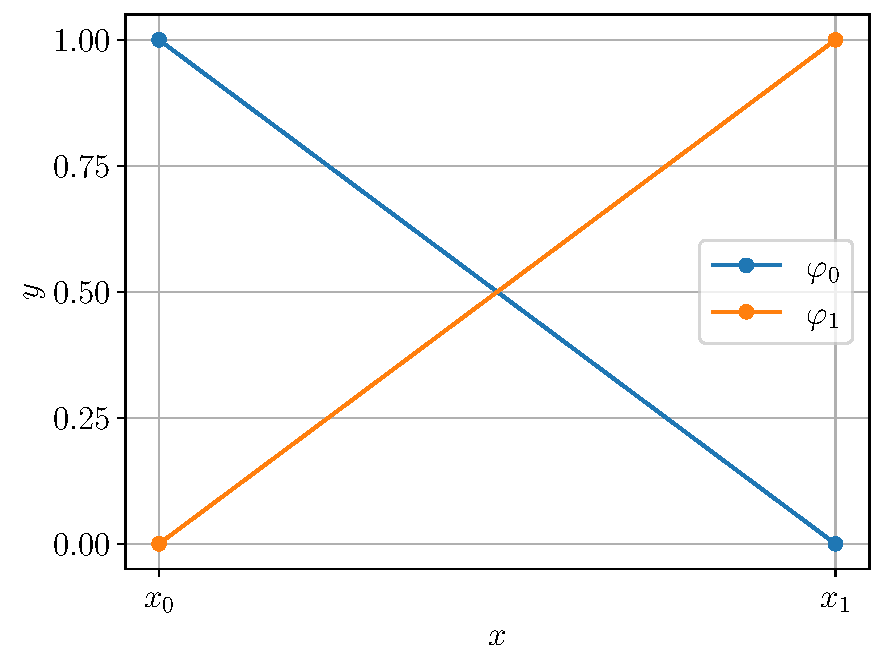
\includegraphics[width=0.7\textwidth]{./cap_mef1d/dados/fig_p1_0/fig}
  \caption{Base nodal para o espaço $P_1([x_0, x_1])$.}
  \label{fig:p1_0}
\end{figure}

Com esta base, toda função $v\in P_1(I)$ pode ser escrita como uma combinação linear das funções $\varphi_0$ e $\varphi_1$ com coeficientes $\alpha_0$ e $\alpha_1$ (\hlemph{graus de liberdade}), i.e.
\begin{equation}\hleq
  v(x) = \alpha_0\varphi_0(x) + \alpha_1\varphi_1(x).
\end{equation}
Além disso, observamos que
\begin{align}
  &\varphi_0(x) = \frac{x-x_1}{x_0-x_1},\\
  &\varphi_1(x) = \frac{x-x_0}{x_1-x_0}.
\end{align}



Uma extensão do espaço $P_1(I)$ é o \hlemph{espaço das funções lineares por partes}. Dado $I = [l_0, l_1]$, $l_0\neq l_1$, consideramos uma partição (\hlemph{malha}) de $I$ com $n+1$ pontos
\begin{equation}
  \mathcal{I} = \{l_0=x_0, x_1, \dotsc, x_n=l_1\}
\end{equation}
e, portanto, com $n$ subintervalos $I_i=[x_{i-1}, x_{i}]$ de comprimento (\hlemph{tamanho da malha}) $h_i = x_i-x_{i-1}$, $i=1, 2, \dotsc, n$. Na malha $\mathcal{I}$ definimos o seguinte \emph{espaço das funções lineares por partes}
\begin{equation}\hleq
  V_h := \{v:~v\in C^0(\mathcal{I}),~v|_{I_i}\in P_1(I_i),~i=1,2,\dotsc,n\}.
\end{equation}
Observamos que \hl{toda função $v\in V_h$ é unicamente determinada por seus valores nodais $\{\alpha_i = v(x_i)\}_{i=0}^n$}. Reciprocamente, \hl{todo conjunto de valores nodas $\{\alpha_i\}_{i=0}^n$ determina unicamente uma função $v\in V_h$}. Desta observação, temos que os \hlemph{valores nodais determinam os graus de liberdade} com a base nodal $\{\varphi_j\}_{j=0}^n$ para $V_h$ definida por
\begin{equation}\hleq
  \varphi_j(x_i) = \left\{
    \begin{array}{ll}
      1 &, i=j,\\
      0 &, i\neq j
    \end{array}
\right.,
\end{equation}
com $i,j=0,1,\dotsc,n$. Ou seja, temos que
\begin{equation}\hleq
    v(x) = \sum_{j=0}^{n}\alpha_j\phi_j(x).
\end{equation}
Podemos verificar que
\begin{equation}
  \varphi_i(x) = \left\{
    \begin{array}{ll}
      (x-x_{i-1})/h_i &, x\in I_i,\\
      (x_{i+1}-x)/h_{i+1} &, x\in I_{i+1},\\
      0 &, \text{noutros casos}
    \end{array}
\right.
\end{equation}
consulte, Figura~\ref{fig:baselinear}. É notável que $\varphi_i(x)$ tem suporte compacto $I_i\cup I_{i+1}$.

\begin{figure}[h!]
  \centering
  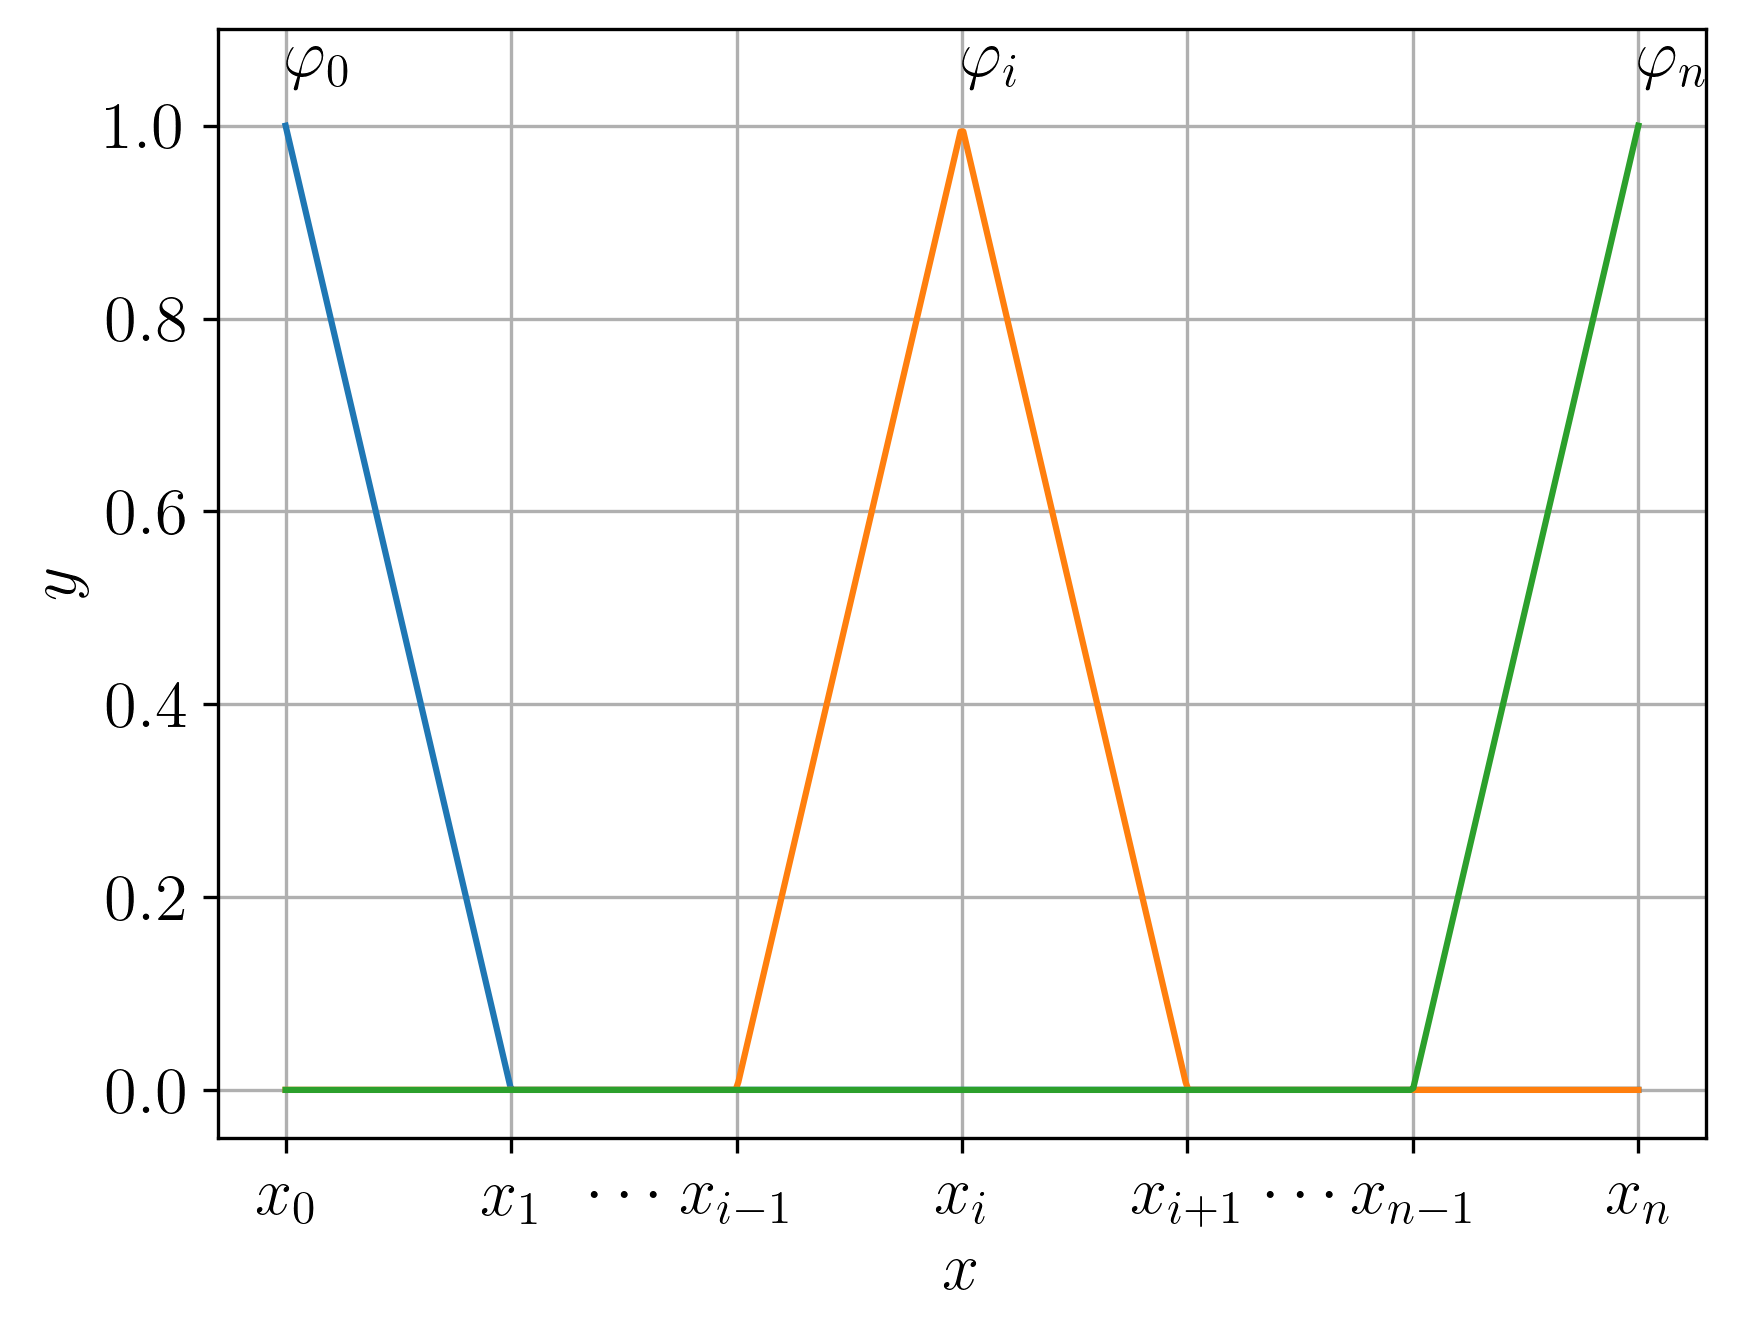
\includegraphics[width=0.7\textwidth]{./cap_mef1d/dados/fig_baselinear/fig}
  \caption{Base nodal para o espaço das funções lineares por parte.}
  \label{fig:baselinear}
\end{figure}

\subsection{Interpolação}
\badgeRevisar

\hl{Interpolação é uma técnica de aproximação de funções}. Dada uma função contínua $f$ em $I=[l_0, l_1]$, definimos o \hlemph{operador de interpolação linear} $\pi: C^0(I)\to V_h$ por
\begin{equation}\hleq
  \pi f (x) = \sum_{j=0}^{n}f(x_j)\varphi_j(x)
\end{equation}
Observamos que $\pi f$ é igual a $f$ nos nodos $x_j$, $j=0, 1, 2, \dotsc, n$. 

\begin{ex}\label{ex:mef1d_interp_lin}
  A Figura~\ref{fig:ex_mef1d_interp_lin} ilustra a interpolação da função $f(x)=3\sen(2\pi x)$ no espaço de elementos finitos $V_h$ das funções lineares por partes com $5$ células.

  \begin{figure}[H]
    \centering
    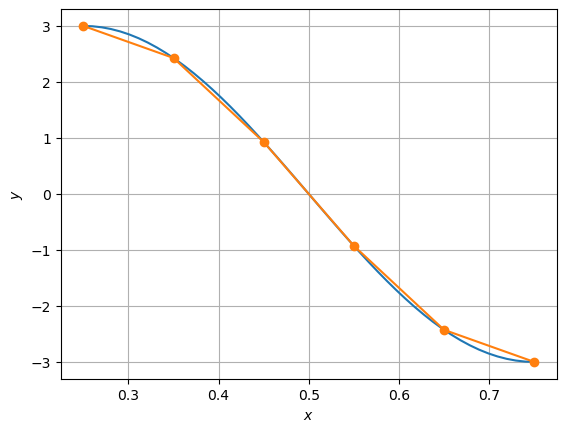
\includegraphics[width=0.8\textwidth]{./cap_mef1d/dados/ex_mef1d_interp_lin/fig}
    \caption{Interpolação linear de $f(x)=3\sen(2\pi x)$ no espaço de elementos finitos $V$.}
    \label{fig:ex_mef1d_interp_lin}
  \end{figure}


\begin{lstlisting}[caption=mef1d\_interp\_lin]
from dolfinx import fem, mesh
import ufl
import numpy as np
from mpi4py import MPI
import matplotlib.pyplot as plt

# malha
l0 = 0.25
l1 = 0.75
domain = mesh.create_interval(MPI.COMM_WORLD,
                              nx = 5,
                              points = [l0, l1])
x = ufl.SpatialCoordinate(domain)

# espaço
V = fem.FunctionSpace(domain, ('P', 1))

# fun
def fun(x, mod):
    return 3.*mod.sin(2.*mod.pi*x)

x = ufl.SpatialCoordinate(domain)
f_expr = fem.Expression(fun(x[0], ufl),
                        V.element.interpolation_points())

# interpolação
pif = fem.Function(V)
pif.interpolate(f_expr)
\end{lstlisting}
\end{ex}

Agora, vamos buscar medir o erro de interpolação, i.e. $f - \pi f$. Para tanto, podemos usar a norma $L^2$ definida por
\begin{equation}
  \|v\|_{L^2(I)} = \left(\int_I v^2\, dx\right)^{1/2}.
\end{equation}
Lembramos que valem a \pmb{desigualdade triangular}\index{desigualdade!triangular}
\begin{equation}
  \|v+w\|_{L^2(I)} \leq \|v\|_{L^2(I)} +  \|w\|_{L^2(I)}
\end{equation}
e a \pmb{desigualdade de Cauchy-Schwarz}\index{desigualdade!de Cauchy-Schwarz}\footnote{Também conhecida como desigualdade de Cauchy–Bunyakovsky–Schwarz. Augustin-Louis Cauchy, 1789 - 1857, matemático francês. Viktor Yakovlevich Bunyakovsky, 1804 - 1889, matemático Russo. Karl Hermann Amandus Schwarz, 1843 - 1921, matemático alemão.}
\begin{equation}\label{eq:Cauchy-Schwarz}
  \int_I vw\,dx \leq \|v\|_{L^2(I)}\|w\|_{L^2(I)},
\end{equation}
para qualquer funções $v,w\in L^2(I)$.

\begin{prop}\normalfont(Erro da interpolação linear)\label{prop:interp_lin}
  O interpolador $\pi f:C^0(I)\to P_1(I)$ satisfaz as estimativas
  \begin{align}
    \|f-\pi f\|_{L^2(I)} &\leq Ch^2\|f''\|_{L^2(I)},\\
    \|(f-\pi f)'\|_{L^2(I)} &\leq Ch\|f''\|_{L^2(I)},
  \end{align}
onde $C$ é uma constante e $h=x_1-x_0$.
\end{prop}
\begin{dem}
  Denotemos o erro de interpolação por $e = f - \pi f$. Do teorema fundamental do cálculo, temos
  \begin{equation}
    e(y) = e(x_0) + \int_{x_0}^y e'(x)\,dx,
  \end{equation}
onde $e(x_0)=f(x_0)-\pi f(x_0) = 0$. Daí, usando a desigualdade de Cauchy-Schwarz~\eqref{eq:Cauchy-Schwarz}, temos
\begin{align}
  e(y) &= \int_{x_0}^y e'\,dx\\
       &\leq \int_{x_0}^y |e'|\,dx\\
       &\leq \int_{I} 1\cdot |e'|\,dx\\
       &\leq \left(\int_{I} 1^2\,dx\right)^{1/2} \left(\int_{I} e'^2\,dx\right)^{1/2}\\
       &= h^{1/2}\left(\int_{I} e'^2\,dx\right)^{1/2},
\end{align}
donde
\begin{equation}
  e(y)^2 \leq h\int_I e'^2\,dx = h\|e'\|_{L^2(I)}^2.
\end{equation}
Então, integrando em $I$ obtemos
\begin{equation}
  \|e\|_{L^2(I)}^2 = \int_I e^2(y)\,dy \leq \int_I h\|e'\|_{L^2(I)}^2\,dy = h^2\|e'\|_{L^2(I)}^2,
\end{equation}
ou seja, temos a seguinte desigualdade
\begin{equation}\label{eq:prop_pif_0}
  \|e\|_{L^2(I)} \leq h\|e'\|_{L^2(I)}.
\end{equation}

Agora, observando que $e(x_0)=e(x_1)=0$, o \pmb{teorema de Rolle}\index{teorema!de Rolle}\footnote{Michel Rolle, 1652 - 1719, matemático francês.} garante a existência de um ponto $\tilde{x}\in I$ tal que $e'(\tilde{x})=0$, donde do teorema fundamental do cálculo e da desigualdade de Cauchy-Schwarz, segue
\begin{align}
  e'(y) &= e'(\tilde{x}) + \int_{\tilde{x}}^y e''\,dx \\
        &= \int_{\tilde{x}}^y e''\,dx\\
        &\leq \int_{I}1\cdot |e''|\,dx\\
        &\leq h^{1/2}\left(\int_I e''^2\right)^{1/2}.
\end{align}
Então, integrando em $I$, obtemos
\begin{equation}\label{eq:prop_pif_1}
  \|e'\|_{L^2(I)}^2 \leq h^2\|e''\|_{L^2(I)}^2,
\end{equation}
a qual, observando que $e'' = f''$, equivale a segunda estimativa procurada, i.e.
\begin{equation}
  \|(f-\pi f)'\|_{L^2(I)} \leq C h \|f''\|_{L^2(I)}.
\end{equation}
Por fim, de \eqref{eq:prop_pif_1} e de \eqref{eq:prop_pif_0}, obtemos a primeira estimativa desejada
\begin{equation}
  \|f - \pi f\|_{L^2(I)} \leq C h^2 \|f''\|_{L^2(I)}.
\end{equation}
\end{dem}

% \begin{ex}\label{ex:esterro_interp_lin}
%   A Figura \ref{fig:ex_esterro_interp_lin} mostra a evolução do erro na norma $L^2$ da interpolação de $f(x)=3\sen(2\pi x)$ no espaço $P_1([0, h)]$ para $h=10^{-5}, 10^{-4}, \cdots, 10^{-1}$.

%   \begin{figure}[h!]
%     \centering
%     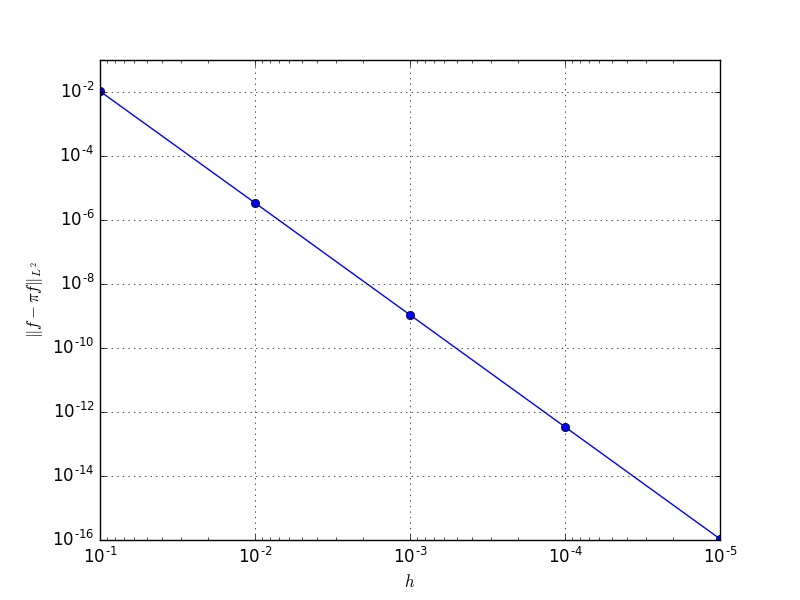
\includegraphics[width=0.8\textwidth]{./cap_mef1d/dados/ex_esterro_interp_lin/ex_esterro_interp_lin}
%     \caption{Erro de interpolação de $f(x)=3\sen(2\pi x)$ no espaço $P_1([0, h])$.}
%     \label{fig:ex_esterro_interp_lin}
%   \end{figure}

% \ifispython
% Com o \fenics, podemos computar os erros de interpolação com o seguinte \href{https://github.com/phkonzen/notas/blob/master/src/MetodoElementosFinitos/cap_mef1d/dados/ex_esterro_interp_lin/ex_esterro_interp_lin.py}{código}:
% \verbatiminput{./cap_mef1d/dados/ex_esterro_interp_lin/ex_esterro_interp_lin.py}
% \fi
% \end{ex}


Vamos, agora, generalizar o resultado da Proposição \ref{prop:interp_lin} para a interpolação no espaço $V_h$ das funções lineares por parte.

% \begin{ex}\label{ex:interp_linpartes}
%   A Figura~\ref{fig:ex_interp_linpartes} ilustra a interpolação da função $f(x)=3\sen(2\pi x)$ no espaço $V_h$ das funções lineares por partes em uma malha uniforme do intervalo $I=[1/4, 3/4]$ com $n=4$ subintervalos ($5$ pontos). 

%   \begin{figure}[h!]
%     \centering
%     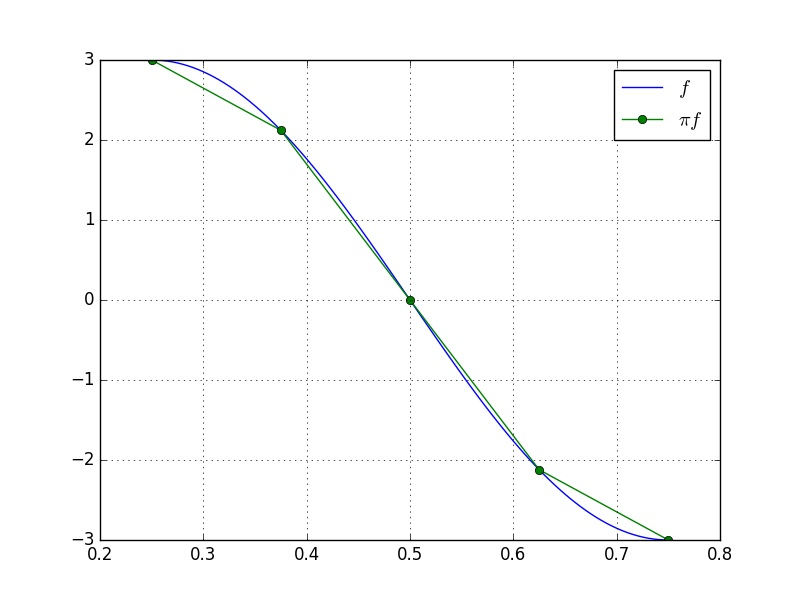
\includegraphics[width=0.8\textwidth]{./cap_mef1d/dados/ex_interp_linpartes/ex_interp_linpartes}
%     \caption{Interpolação linear de $f(x)=3\sen(2\pi x)$ no espaço $V_h$ das funções lineares por partes sobre uma malha com $5$ pontos.}
%     \label{fig:ex_interp_linpartes}
%   \end{figure}

% \ifispython
% Com o \fenics, podemos computar a função interpolada $\pi f$ com o seguinte \href{https://github.com/phkonzen/notas/blob/master/src/MetodoElementosFinitos/cap_mef1d/dados/ex_interp_linpartes/ex_interp_linpartes.py}{código}:
% \verbatiminput{./cap_mef1d/dados/ex_interp_linpartes/ex_interp_linpartes.py}
% \fi
% \end{ex}

O seguinte resultado fornece uma estimativa do erro de interpolação em relação ao tamanho $h_i$ de cada elemento da malha.

\begin{prop}\label{prop:interp_linpartes}
  O interpolador $\pi f$ satisfaz as estimativas
  \begin{align}
    \|f-\pi f\|_{L^2(I)}^2 &\leq C\sum_{i=1}^n h_i^4\|f''\|_{L^2(I)}^2,\\
    \|(f-\pi f)'\|_{L^2(I)}^2 &\leq C\sum_{i=1}^n h_i^2\|f''\|_{L^2(I)}^2.\\
  \end{align}
\end{prop}
\begin{dem}
  Ambas desigualdades seguem da desigualdade triangular e da Proposição~\ref{prop:interp_lin}. Por exemplo, para a primeira desigualdade, temos
  \begin{align}
    \|f - \pi f\|_{L^2(I)}^2 &\leq \sum_{i=1}^n \|f - \pi f\|_{L^2(I_i)}^2\\
    &\leq \sum_{i=1}^n Ch_i^4 \|f''\|_{L^2(I_i)}^2.
  \end{align}
\end{dem}

\subsection{Projeção $L^2$}\label{subsec:projecao_1d}
\badgeRevisar

Dada uma função $f\in L^2(I)$, definimos o \hlemph{operador de projeção $L^2$} $P_h:L^2(I)\to V_h$ por
\begin{equation}\label{eq:proj_def}\hleq
  \int_I (f-P_hf)v\,dx=0,\quad\forall v\in V_h.
\end{equation}

Como $V_h$ é um espaço de dimensão finita, a condição \eqref{eq:proj_def} é equivalente a
\begin{equation}
  \int_I (f-P_hf)\varphi_i\,dx=0,\quad i=0, 1, \cdots, n,
\end{equation}
onde $\varphi_i$ é a $i$-ésima função base de $V_h$. Além disso, como $P_hf\in V_h$, temos
\begin{equation}
  P_hf = \sum_{j=0}^n\xi_j\varphi_j,
\end{equation}
onde $\xi_j$, $j=0, 1, \dotsc, n$, são $n+1$ incógnitas a determinar. Logo,
\begin{gather}
  \int_I (f-P_hf)\varphi_i\,dx=0 \\
  \int_I f\varphi_i\,dx = \int_I P_hf\varphi_i\,dx\\
  \int_I f\varphi_i\,dx = \int_I \left(\sum_{j=0}^n \xi_j\varphi_j\right)\varphi_i\,dx\\
  \sum_{j=0}^n \xi_j\int_I\varphi_j\varphi_i\,dx = \int_I f\varphi_i\,dx,\label{eq:proj_siseq}
\end{gather}
para $i=0, 1, \dotsc, n$.

Observamos que \eqref{eq:proj_siseq} consiste em um sistema de $n+1$ equações lineares para as $n+1$ incógnitas $\xi_j$, $j=0, 1, \dotsc, n$. Este, por sua vez, pode ser escrito na seguinte forma matricial
\begin{equation}\label{eq:proj_sis}\hleq
  M\xi = b,
\end{equation}
onde \hl{$M = [m_{i,j}]_{i,j=0}^{n+1}$ é chamada de \emph{matriz de massa}}
\begin{equation}\hleq
  m_{i,j} = \int_I\varphi_j\varphi_i\,dx
\end{equation}
e \hl{$b = (b_0, b_1, \dotsc, b_n)$ é chamado de \emph{vetor de carregamento}}
\begin{equation}\hleq
  b_i = \int_I f\varphi_i\,dx.
\end{equation}

Ou seja, \hl{a projeção $L^2$ de $f$ no espaço $V_h$ é}
\begin{equation}\hleq
  P_hf = \sum_{j=0}^n\xi_j\varphi_j,
\end{equation}
\hl{onde $\xi = (\xi_0, \xi_1, \dotsc, \xi_n)$ é solução do sistema {\eqref{eq:proj_sis}}}.

\begin{ex}\label{ex:mef1d_proj}
  A Figura~\ref{fig:ex_mef1d_proj} ilustra a projeção $L^2$ da função $f(x)=3\sen(2\pi x)$ no espaço $V_h$ das funções lineares por partes em uma malha uniforme do intervalo $I=[1/4, 3/4]$ com $n=4$ subintervalos ($5$ células).

  \begin{figure}[h!]
    \centering
    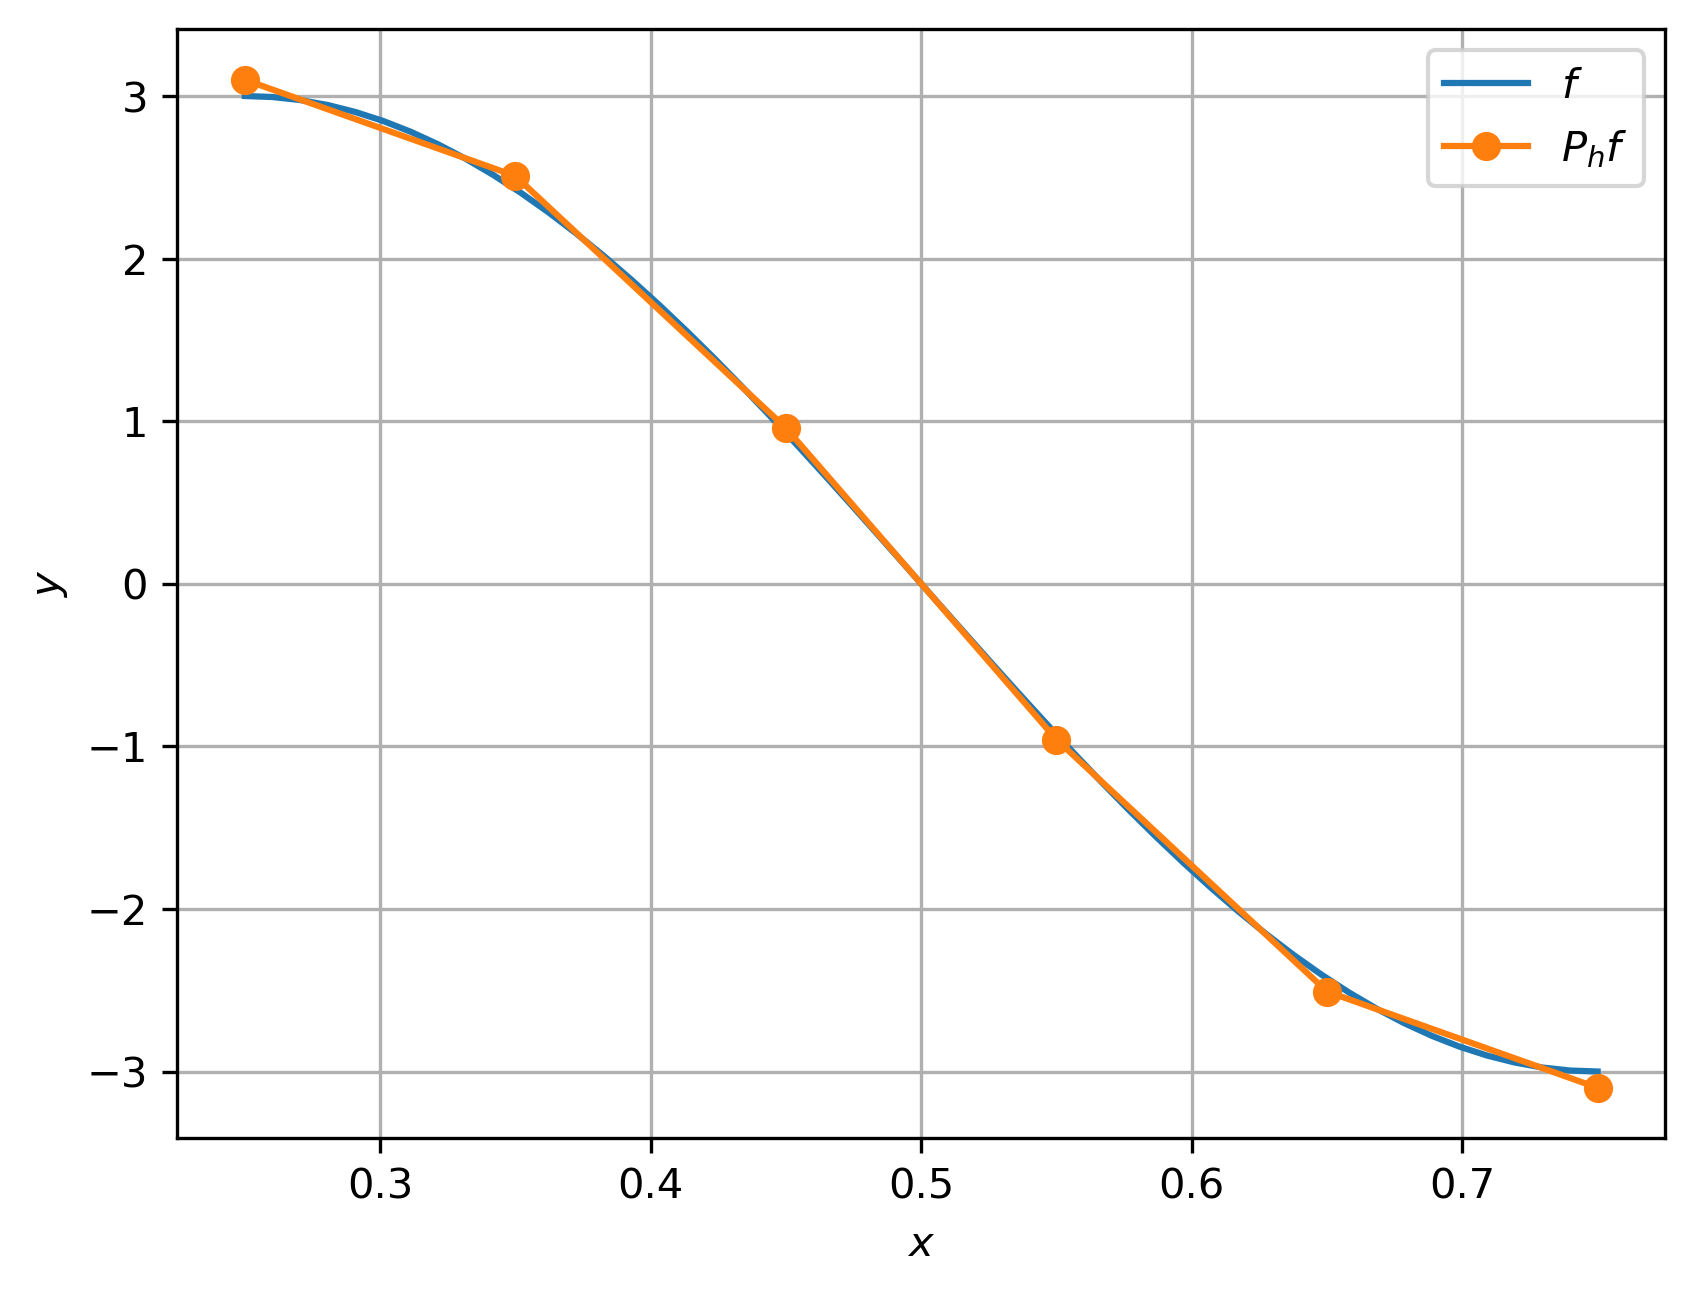
\includegraphics[width=0.8\textwidth]{./cap_mef1d/dados/ex_mef1d_proj/fig}
    \caption{Projeção $L^2$ de $f(x)=3\sen(2\pi x)$ no espaço $V_h$ das funções lineares por partes sobre uma malha com $5$ células.}
    \label{fig:ex_mef1d_proj}
  \end{figure}

\begin{lstlisting}[caption=ex\_mef1d\_proj.py]
from dolfinx import fem, mesh
from dolfinx.fem.petsc import LinearProblem
import ufl
from mpi4py import MPI

# malha
l0 = 0.25
l1 = 0.75
domain = mesh.create_interval(MPI.COMM_WORLD,
                              nx=5,
                              points=[l0, l1])
x = ufl.SpatialCoordinate(domain)

# espaço
V = fem.functionspace(domain, ("P", 1))

# fun
f = 3.*ufl.sin(2.*ufl.pi*x[0])

# project f
u = ufl.TrialFunction(V)
v = ufl.TestFunction(V)
a =  ufl.dot(u, v) * ufl.dx
L = ufl.dot(f, v) * ufl.dx
problem = LinearProblem(a, L, bcs=[])
Phf = problem.solve()
\end{lstlisting}
\end{ex}

O próximo teorema mostra que $P_h f$ é a função que melhor aproxima $f$ dentre todas as funções do espaço $V_h$.

\begin{teo}(\normalfont{A melhor aproximação.})\label{teo:melhor_aprox}
  A projeção $L^2$ satisfaz
  \begin{equation}
    \|f-P_hf\|_{L^2(I)} \leq \|f - v\|_{L^2(I)},\quad\forall v\in V_h.
  \end{equation}
\end{teo}
\begin{dem}
  Dado $v\in V_h$, temos
  \begin{align}
    \|f-P_hf\|_{L^2(I)}^2 &= \int_I |f-P_hf|^2\,dx\\
    &= \int_I (f-P_hf)(f-v+v-P_hf)\,dx\\
    &= \int_I(f-P_hf)(f-v)\,dx + \int_I(f-P_hf)(v-P_hf)\,dx\\
    &= \int_I (f-P_hf)(f-v)\,dx\\
    &\leq \|f-P_hf\|_{L^2(I)}\|f-v\|_{L^2(I)},
  \end{align}
donde segue o resultado.
\end{dem}

O próximo teorema fornece uma estimativa \textit{a-priori} do erro $\|f-P_h f\|_{L^2(I)}$ em relação ao tamanho da malha.

\begin{teo}\label{teo:erro_proj_1d}
  A projeção $L^2$ satisfaz
  \begin{equation}
    \|f-P_hf\|_{L^2(I)}^2 \leq C\sum_{i=1}^n h_i^4\|f''\|_{L^2(I_i)}^2.
  \end{equation}
\end{teo}
\begin{dem}
  Tomando a interpolação $\pi f \in V_h$, temos do Teorema da melhor aproximação (Teorema \ref{teo:melhor_aprox}) e da estimativa do erro de interpolação (Proposição \ref{prop:interp_linpartes}) que
  \begin{align}
    \|f - P_hf\|_{L^2(I)}^2 &\leq \|f-\pi f\|_{L^2(I)}^2\\
    &\leq C\sum_{i=1}^n h_i^4\|f''\|_{L^2(I_i)}^2.
  \end{align}
\end{dem}

% \begin{ex}\label{ex:esterro_proj}
%   A Figura \ref{fig:ex_esterro_proj} mostra a evolução do erro na norma $L^2$ da projeção de $f(x)=3\sen(2\pi x)$ no espaço $V_h$ em malhas uniformes de $h=10^{-5}, 10^{-4}, \cdots, 10^{-1}$ no intervalo $[1/4, 3/4]$.

%   \begin{figure}[h!]
%     \centering
%     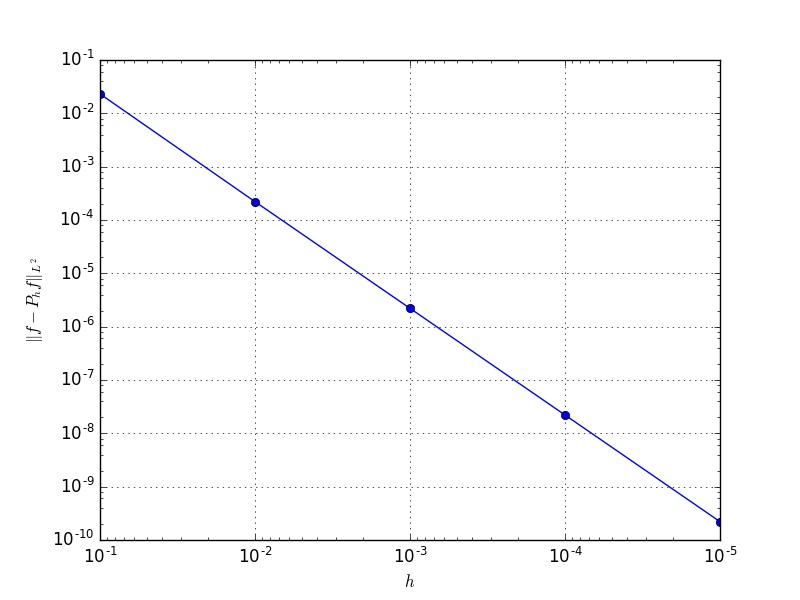
\includegraphics[width=0.8\textwidth]{./cap_mef1d/dados/ex_esterro_proj/ex_esterro_proj}
%     \caption{Erro de interpolação de $f(x)=3\sen(2\pi x)$ no espaço $V_h$.}
%     \label{fig:ex_esterro_proj}
%   \end{figure}

% \ifispython
% Com o \fenics, podemos computar os erros de projeção com o seguinte \href{https://github.com/phkonzen/notas/blob/master/src/MetodoElementosFinitos/cap_mef1d/dados/ex_esterro_proj/ex_esterro_proj.py}{código}:
% \verbatiminput{./cap_mef1d/dados/ex_esterro_proj/ex_esterro_proj.py}
% \fi
% \end{ex}

\subsection{Exercícios}
\badgeRevisar

\begin{exer}
  Faça um código para verificar a segunda estimativa da Proposição~\ref{prop:interp_lin} no caso da interpolação da função $f(x) = 3\sen(2\pi x)$ no espaço $P_1$ das funções lineares.
\end{exer}
\begin{resp}
  \badgeConstrucao
\end{resp}


\begin{exer}
  Faça um código para verificar as estimativas da Proposição~\ref{prop:interp_linpartes} no caso da interpolação da função $f(x) = 3\sen(2\pi x)$ no espaço $V_h$ das funções lineares por partes.
\end{exer}
\begin{resp}
  \badgeConstrucao
\end{resp}

\begin{exer}
  Faça um código para computar a projeção $L^2$ $P_hf$ da função $f(x) = x - cos(x)$ no espaço $V_h$ das funções lineares por partes em uma malha com $10$ células no intervalo $I = [0, \pi]$. Faça o esboço dos gráficos de $f$ e $P_hf$ e compute o erro $\|f-P_hf\|_{L^2(I)}$.
\end{exer}

\subsubsection{Respostas}

\shipoutAnswer

\section{Problema Modelo}\label{cap_mef1d_sec_modelo}
\badgeRevisar

Nesta seção, discutimos sobre a aplicação do método de elementos finitos para o seguinte problema de valor de contorno: encontrar $u$ tal que
\begin{align}
  -u'' &= f,\quad x\in I=[0,L],\label{eq:prob_eq}\\
  u(0) &= u(L) = 0,\label{eq:prob_bc}
\end{align}
onde $f$ é uma função dada.

\subsection{Formulação Fraca}
\badgeRevisar

A derivação de um método de elementos finitos inicia-se da formulação fraca do problema em um espaço de funções apropriado. No caso do problema \eqref{eq:prob_eq}-\eqref{eq:prob_bc}, tomamos o espaço
\begin{equation}
  V_0 = \{v\in H^1(I):~v(0)=v(1)=0\}.
\end{equation}
Ou seja, se $v\in H^1(I)$, então $\|v\|_{L^2(I)}<\infty$, $\|v'\|_{L^2(I)}<\infty$, bem como $v$ satisfaz as condições de contorno do problema.

A formulação fraca é, então, obtida multiplicando-se a equação \eqref{eq:prob_eq} por uma função teste $v\in V_0$ (arbitrária) e integrando-se por partes, i.e.
\begin{align}
  \int_I fv\,dx &= -\int_I u''v\,dx\\
  &= \int_I u'v'\,dx - u'(L)v(L) + u'(0)v(0)\\
\end{align}
Donde, das condições de contorno, temos
\begin{equation}
  \int_I u'v'\,dx = \int_I fv\,dx.
\end{equation}

Desta forma, o problema fraco associado a \eqref{eq:prob_eq}-\eqref{eq:prob_bc} lê-se: encontrar $u\in V_0$ tal que
\begin{equation}\label{eq:modelo_ffraca}
  a(u,v) = L(v),\quad\forall v\in V_0,
\end{equation}
onde
\begin{align}
  a(u,v) &= \int_I u'v'\,dx\label{eq:modelo_fbilinear}\\
  L(v) &= \int_I fv\,dx,\label{eq:modelo_flinear}
\end{align}
são chamadas de forma bilinear e forma linear, respectivamente.

\subsection{Formulação de Elementos Finitos}
\badgeRevisar

Uma formulação de elementos finitos é um aproximação do problema fraco \eqref{eq:modelo_ffraca} em um espaço de dimensão finita. Aqui, vamos usar o espaço $V_{h,0}$ das funções lineares por partes em $I$ que satisfazem as condições de contorno, i.e.
\begin{equation}
  V_{h,0} = \{v\in V_h:~v(0)=v(L)=0\}.
\end{equation}

Então, substituindo o espaço $V_0$ pelo subespaço $V_{h,0}\subset V_0$ em \eqref{eq:modelo_ffraca}, obtemos o seguinte problema de elementos finitos: encontrar $u_h\in V_{h,0}$ tal que
\begin{equation}\label{eq:modelo_fem}
  a(u_h,v) = L(v),\quad\forall v\in V_{h,0}.
\end{equation}

\begin{obs}
  A formulação de elementos finitos não é única, podendo-se trabalhar com outros espaços de funções. No caso em que o espaço da solução é igual ao espaço das funções testes, a abordagem é chamada de método de Galerkin\footnote{Boris Grigoryevich Galerkin, matemático e engenheiro soviético. Fonte: \href{https://pt.wikipedia.org/wiki/Boris_Galerkin}{Wikipédia}.}.
\end{obs}

Observemos que o problema \eqref{eq:modelo_fem} é equivalente a: encontrar $u_h\in V_{h,0}$ tal que
\begin{equation}
  a(u_h,\varphi_i) = L(\varphi_i),\quad i=1, \dotsc, n-1,
\end{equation}
onde $\varphi_i$, $i=1,\dotsc,n-1$, são as funções base de $V_{h,0}$. Então, como $u_h\in V_{h,0}$, temos
\begin{equation}
  u_h = \sum_{j=1}^{n-1}\xi_j\varphi_j,
\end{equation}
onde $\xi_j$, $j=1,2,\dotsc,n-1$, são incógnitas a determinar. I.e., ao computarmos $\xi_j$, $j=1,2,\dotsc,n-1$, temos obtido a solução $u_h$ do problema de elementos finitos \ref{eq:modelo_fem}.

Agora, da forma bilinear \eqref{eq:modelo_fbilinear}, temos
\begin{align}
  a(u_h,\varphi_i) &= a\left(\sum_{j=1}^{n-1}\xi_j\varphi_j,\varphi_i\right)\\
  &= \sum_{j=1}^{n-1}\xi_j a(\varphi_j,\varphi_i).
\end{align}

Daí, o problema \eqref{eq:modelo_fem} é equivalente a resolvermos o seguinte sistema de equações lineares
\begin{equation}\label{eq:modelo_fem_sis}
  A\xi = b,
\end{equation}
onde $A = [a_{i,j}]_{i,j=1}^{n-1}$ é a matriz de rigidez com
\begin{equation}
  a_{i,j} = a(\varphi_j,\varphi_i) = \int_{I}\varphi_j'\varphi_i'\,dx,
\end{equation}
$\xi = (\xi_1,\xi_2,\dotsc,\xi_{n-1})$ é o vetor das incógnitas e $b = (b_{i})_{i=1}^{n-1}$ é o vetor de carregamento com
\begin{equation}
  b_i = L(\varphi_i) = \int_If \varphi_i\,dx.
\end{equation}

\begin{ex}\label{ex:mef1d_modelo}
  Consideramos o problema \eqref{eq:prob_eq}-\eqref{eq:prob_bc} com $f\equiv 1$ e $L=1$, i.e.
  \begin{align}
    -u'' &= 1,\quad x\in I=[0,1],\label{eq:ex_modelo_eq}\\
    u(0) &= u(1) = 0.\label{eq:ex_modelo_bc}
  \end{align}
Neste caso, a solução analítica $u(x) = -x^2/2+x/2$ pode ser facilmente obtida por integração.

Agora, vamos computar uma aproximação de elementos finitos no espaço das funções lineares por partes $V_{h,0} = \{v\in P_1(I);~v(0)=v(1)=0\}$ construído numa malha uniforme de $5$ células no intervalo $I=[0, 1]$. Para tanto, consideramos o problema fraco: encontrar $u\in V_0 = \{v\in H^1(I);~v(0)=v(L)=0\}$ tal que
\begin{equation}
  a(u, v) = L(v),
\end{equation}
onde
\begin{equation}
  a(u, v) = \int_I u'v'\,dx,\quad L(v)=\int_I fv\,dx.
\end{equation}

Então, a formulação de elementos finitos associada, lê-se: encontrar $u_h\in V_{h,0}$ tal que
\begin{equation}
  a(u_h, v_h) = L(v_h),\quad\forall v_h\in V_{h,0}.
\end{equation}
A Figura \ref{fig:ex_modelo} apresenta o esboço dos gráficos da solução analítica $u$ e da sua aproximação de elementos finitos $u_h$.

\begin{figure}[h!]
  \centering
  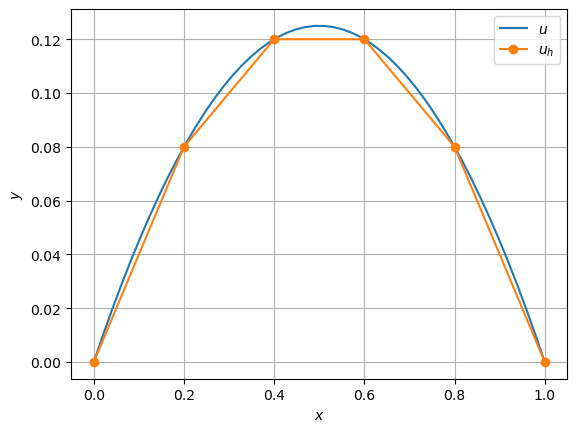
\includegraphics[width=0.8\textwidth]{./cap_mef1d/dados/ex_mef1d_modelo/fig}
  \caption{Esboço dos gráficos das soluções referentes ao Exemplo~\ref{ex:mef1d_modelo}.}
  \label{fig:ex_mef1d_modelo}
\end{figure}

\begin{lstlisting}[caption=ex\_mef1d\_modelo.py]
from mpi4py import MPI

# malha
from dolfinx import mesh
domain = mesh.create_unit_interval(MPI.COMM_WORLD,
                                   nx = 5)
# espaço
from dolfinx import fem
V = fem.functionspace(domain, ('P', 1))

# condição de contorno
import numpy as np
uD = fem.Function(V)
uD.interpolate(lambda x: np.full(x.shape[1], 0.))

tdim = domain.topology.dim
fdim = tdim - 1
domain.topology.create_connectivity(fdim, tdim)
boundary_facets = mesh.exterior_facet_indices(domain.topology)
boundary_dofs = fem.locate_dofs_topological(V, fdim,
                                            boundary_facets)
bc = fem.dirichletbc(uD, boundary_dofs)

# problema mef
import ufl
from dolfinx import default_scalar_type
from dolfinx.fem.petsc import LinearProblem
u = ufl.TrialFunction(V)
v = ufl.TestFunction(V)

f = fem.Constant(domain, default_scalar_type(1.))

a = ufl.dot(ufl.grad(u), ufl.grad(v)) * ufl.dx
L = f * v * ufl.dx

problem = LinearProblem(a, L, bcs=[bc])
uh = problem.solve()
\end{lstlisting}
\end{ex}

\subsection{Estimativa \textit{a Priori}}
\badgeRevisar

Existem dois tipos de \hl{\emph{estimativas do erro} $e := u - u_h$}. \hl{Estimativas \textbf{\textit{a priori}}, são aquelas em que o erro é dado em relação da solução $u$}, enquanto que nas \hl{estimativas \textbf{\textit{a posteriori}} o erro é expresso em relação a solução de elementos finitos $u_h$}.

\begin{teo}\normalfont{(\hl{Ortogonalidade de Galerkin}.)}\label{teo:ortogonalidade_de_Galerkin}
  A solução de elementos finitos $u_h$ de \eqref{eq:modelo_fem} satisfaz a seguinte propriedade de ortogonalidade
  \begin{equation}
    a(u-u_h,v) := \int_I (u-u_h)'v'\,dx = 0,\quad v\in V_{h,0},
  \end{equation}
onde $u$ é a solução de \eqref{eq:modelo_ffraca}.
\end{teo}
\begin{dem}
  De \eqref{eq:modelo_fem}, \eqref{eq:modelo_ffraca} e lembrando que $V_{h,0}\subset V_0$, temos
  \begin{equation}
    a(u,v) = L(v) = a(u_h,v) \Rightarrow a(u-u_h, v) = 0,
  \end{equation}
para todo $v\in V_{h,0}$.
\end{dem}

\begin{teo}\normalfont{(\hl{A melhor aproximação}.)}\label{teo:fem1d_melhor_aprox}
  A solução de elementos finitos $u_h$ dada por \eqref{eq:modelo_fem} satisfaz a seguinte propriedade de melhor aproximação
  \begin{equation}
    \|(u-u_h)'\|_{L^2(I)} \leq \|(u-v)'\|_{L^2(I)},\quad v\in V_{h,0},\label{eq:modelo_melhor_aprox}
  \end{equation}
onde $u$ é a solução de \eqref{eq:modelo_ffraca}.
\end{teo}
\begin{dem}
  Escrevendo $u-u_h = u-v+v-u_h$ para qualquer $v\in V_{h,0}$ e usando a ortogonalidade de Galerkin (Teorema \ref{teo:ortogonalidade_de_Galerkin}), temos
  \begin{align}
    \|(u-u_h)'\|_{L^2(I)}^2 &= \int_{I} (u-u_h)'(u-u_h)'\,dx\\
    &= \int_I (u-u_h)'(u-v+v-u_h)'\,dx\\
    &= \int_I (u-u_h)'(u-v)'\,dx + \int_I (u-u_h)'(v-u_h)'\,dx\\
    &= \int_I (u-u_h)'(u-v)'\,dx\\
    &\leq \|(u-u_h)'\|_{L^2(I)}\|(u-v)'\|_{L^2(I)}.
  \end{align}
\end{dem}

\begin{teo}\normalfont{(\hl{Estimativa \textit{a priori}}.)}
  O erro em se aproximar a solução $u$ de \eqref{eq:modelo_ffraca} pela solução de elementos finitos $u_h$ dada por \eqref{eq:modelo_fem} satisfaz a seguinte estimativa \textit{a priori}
\begin{equation}
  \|(u-u_h)'\|_{L^2(I)}^2 \leq C\sum_{i=1}^n h_i^2\|u''\|_{L^2(I_i)}^2.
\end{equation}
\end{teo}
\begin{dem}
  Tomando $v = \pi u$ no teorema da melhor aproximação (Teorema \ref{teo:fem1d_melhor_aprox}), obtemos
  \begin{equation}
    \|(u-u_h)'\|_{L^2(I)} \leq \|(u-\pi u)'\|_{L^2(I)}.
  \end{equation}
Daí, da estimativa do erro de interpolação (Proposição \ref{prop:interp_linpartes}), temos
\begin{equation}
  \|(u-u_h)'\|_{L^2(I)}^2 \leq C\sum_{i=1}^n h_i^2\|u''\|_{L^2(I_i)}^2.
\end{equation}
\end{dem}

\begin{ex}\label{ex:modelo_estapriori}
  A Figura \ref{fig:ex_modelo_estapriori} apresenta o esboço da evolução do erro $\|(u - u_h)'\|_{L^2(I)}$ da solução de elementos finitos do problema \eqref{eq:ex_modelo_eq}-\eqref{eq:ex_modelo_bc} para malhas uniformes com $n=2, 4, 8, \ldots, 128$ células.

\begin{figure}[h!]
  \centering
  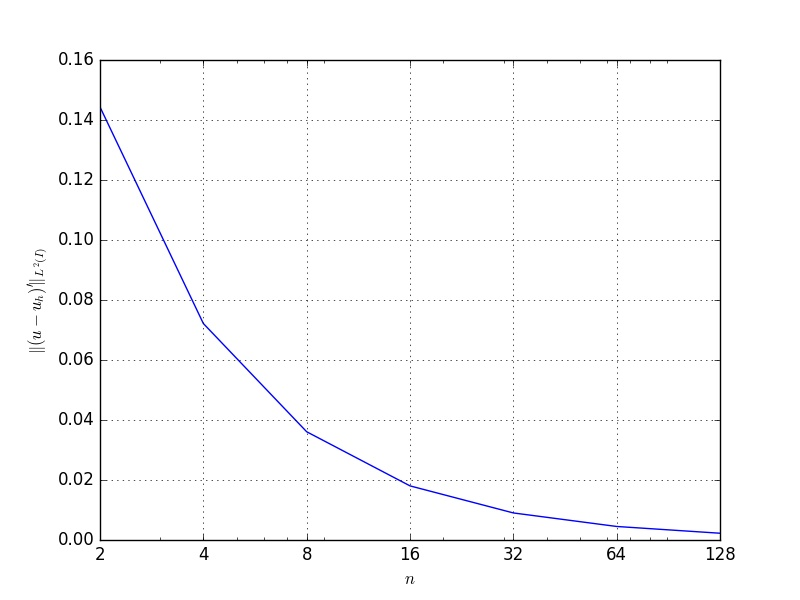
\includegraphics[width=0.8\textwidth]{./cap_mef1d/dados/ex_modelo_estapriori/ex_modelo_estapriori}
  \caption{Esboço dos gráficos das soluções referentes ao Exemplo \ref{ex:modelo_estapriori}.}
  \label{fig:ex_modelo_estapriori}
\end{figure}

\ifispython
Com o \fenics, a computação do problema de elementos finitos pode ser feita com o seguinte \href{https://github.com/phkonzen/notas/blob/master/src/MetodoElementosFinitos/cap_mef1d/dados/ex_modelo_estapriori/ex_modelo_estapriori.py}{código}:
\verbatiminput{./cap_mef1d/dados/ex_modelo_estapriori/ex_modelo_estapriori.py}
\fi
\end{ex}

\subsection{Estimativa \textit{a Posteriori}}
\badgeRevisar

Aqui, vamos obter uma estimativa \textit{a posteriori} para o erro $e = u - u_h$ da solução de elementos finitos $u_h$ do problema \eqref{eq:prob_eq}-\eqref{eq:prob_bc}.

\begin{teo}\label{teo:fem_est_a_posteriori}
  A solução de elementos finitos $u_h$ satisfaz
  \begin{equation}
    \|(u-u_h)'\|_{L^2(I)}^2 \leq C\sum_{i=1}^n \eta_i^2(u_h),
  \end{equation}
onde $\eta_i(u_h)$ é chamado de elemento residual e é dado por
\begin{equation}
  \eta_i(u_h) = h_i\|f - u_h''\|_{L^2(I_i)}.
\end{equation}
\end{teo}
\begin{dem}
  Tomando $e = u - u_h$ e usando a ortogonalidade de Galerkin (Teorema \ref{teo:ortogonalidade_de_Galerkin}) temos
  \begin{equation}
    \|e'\|_{L^2(I)}^2 = \int_I e'(e-\pi e)'\,dx = \sum_{i=1}^n\int_{I_i} e'(e-\pi e)'\,dx.
  \end{equation}
  Então, aplicando integração por partes
  \begin{equation}
    \|e'\|_{L^2(I)}^2 = \sum_{i=1}^n\int_{I_i}(-e'')(e-\pi e)\,dx + [e'(e-\pi e)]_{x_{i-1}}^{x_i}.
  \end{equation}
  Daí, observando que $e-\pi e = 0$ nos extremos dos intervalos $I_i$ e que $-e'' = -(u-u_h)'' = -u'' + u_h'' = f + u_h''$, temos
  \begin{equation}
    \|e'\|_{L^2(I)}^2 = \sum_{i=1}^n\int_{I_i}(f+u_h'')(e-\pi e)\,dx.
  \end{equation}
  Agora, usando as desigualdades de Cauchy-Schwarz e a estimativa padrão de interpolação \eqref{eq:prop_pif_0}, obtemos
  \begin{align}
    \|e'\|_{L^2(I)}^2 &\leq \sum_{i=1}^n\|f+u_h\|_{L^2(I_i)}\|e-\pi e\|_{L^2(I_i)}\,dx\\
    &\leq C\sum_{i=1}^nh_i\|f+u_h\|_{L^2(I_i)}\|e'\|_{L^2(I_i)}\\
    &\leq C\left(\sum_{i=1}^n h_i^2\|f+u_h\|_{L^2(I_i)}^2\right)^{1/2}\left(\sum_{i=1}^n \|e'\|_{L^2(I_i)}^2\right)^{1/2}\\
    &= C\left(\sum_{i=1}^n h_i^2\|f+u_h\|_{L^2(I_i)}^2\right)^{1/2}\|e'\|_{L^2(I)},
  \end{align}
  donde segue o resultado desejado.
\end{dem}

\begin{obs}
  No caso da solução de elementos finitos no espaço das funções lineares por partes, temos $u_h'' = 0$. Logo, o elemento residual se resume em $\eta_i(u_h) = h_i\|f\|_{L^2(I_i)}$.
\end{obs}

\subsection{Exercícios}
\badgeRevisar

\begin{exer}\label{exer:dc}
  Obtenha uma aproximação por elementos finitos lineares por partes da solução de
  \begin{align}
    &-u'' + u = 2\sen x,\quad \forall x\in (-\pi, \pi),\\
    &u(-\pi)=u(\pi)=0.
  \end{align}
\end{exer}
\begin{resp}
  \ifispython
  \href{https://github.com/phkonzen/notas/blob/master/src/MetodoElementosFinitos/cap_mef1d/dados/exer_dc/exer_dc.py}{Código} FENiCS.
  \fi
\end{resp}

\subsubsection{Respostas}

\shipoutAnswer


\section{Condições de Contorno}\label{cap_mef1d_sec_cc}
\badgeRevisar

Nesta seção, vamos discutir sobre \hl{soluções de elementos finitos para a equações diferencial}
\begin{equation}\hleq
  -u'' = f,\quad x\in I=[0, L],
\end{equation}
\hl{com diferentes condições de contorno}.

\subsection{Condições de Dirichlet}
\badgeRevisar

Consideramos o seguinte \hl{problema com condições de contorno de Dirichlet}{\dirichlet}: encontrar $u$ tal que
\begin{align}
  &-u'' = f,\quad \forall x\in I=[0, L],\label{eq:cc_d_eq}\\
  &u(0) = u_0,\quad u(L) = u_L,\label{eq:cc_d_bc}
\end{align}
com $u_0$, $u_L$ e $f$ dados.

Tomando uma função teste $v\in \hleq{V_0 := H^1_0(I):=\{v\in H^1(I);~v(0)=v(L)=0\}}$ e multiplicando-a em \eqref{eq:cc_d_eq}, obtemos
\begin{equation}
  - \int_I u''v\,dx = \int_I fv\,dx.
\end{equation}
Aplicando a integração por partes, temos
\begin{equation}
  \int_I u'v'\,dx = \int_I fv\,dx.
\end{equation}
Desta forma, definimos o seguinte \hlemph{problema fraco} associado: encontrar $u\in \hleq{V := \{v\in H^1(I);~v(0)=u_0,~v(L)=v_L\}}$ tal que
\begin{align}\hleq
  a(u,v) = L(v),\quad\forall v\in V_0,
\end{align}
onde $a(u,v)$ é a forma bilinear
\begin{equation}
  a(u,v) = \int_I u'v'\,dx
\end{equation}
e $L(v)$ é a forma linear
\begin{equation}
  L(v) = \int_I fv\,dx.
\end{equation}

\begin{ex}\label{ex:mef1d_dirichlet}
  Consideramos o problema
  \begin{align}
    &-u'' = 1,\quad x\in I=[0,1],\label{eq:ex_cc_d_eq}\\
    &u(0) = 1/2,\quad u(1) = 1.\label{eq:ex_cc_d_bc}
  \end{align}
Sua solução analítica é $u(x) = -x^2/2+x+1/2$. 

Para obtermos uma aproximação de elementos finitos, consideramos o seguinte problema fraco: encontrar $u\in V := \{v\in H^1(I);~v(0)=1/2,~v(1)=1\}$ tal que
\begin{equation}
  a(u,v) = L(v),
\end{equation}
para todo $v\in V_0 = \{v\in H^1(I);~v(0)=v(1)=0\}$, onde
\begin{align}
  &a(u, v) = \int_I u'v'\,dx,\\
  &L(v) = \int_I fv\,dx.
\end{align}

Então, o problema de elementos finitos no espaço das funções lineares por partes lê-se: encontrar $u_h\in V_h = \{v\in P_1(I);~v(0)=1/2,~v(1)=1\}$ tal que
\begin{equation}
  a(u_h, v_h) = L(v_h),
\end{equation}
para todo $v_h\in V_{h,0} = \{v\in H^1(I);~v(0)=v(1)=0\}$.

% A Figura \ref{fig:ex_cc_d} apresenta o esboço dos gráficos da solução analítica $u$ e da sua aproximação de elementos finitos $u_h$, esta construída no espaço dos polinômios lineares por partes sobre uma malha uniforme de $5$ células.

% \begin{figure}[h!]
%   \centering
%   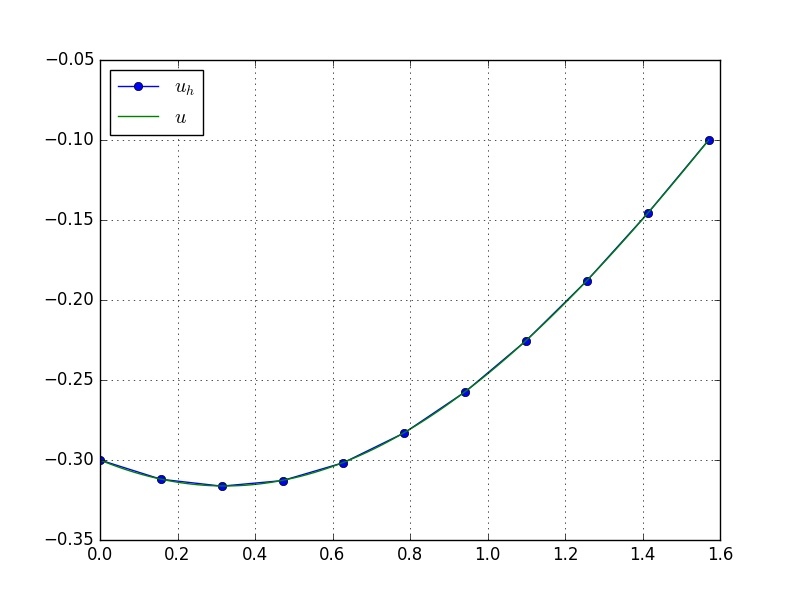
\includegraphics[width=0.8\textwidth]{./cap_mef1d/dados/ex_cc_d/ex_cc_d}
%   \caption{Esboço dos gráficos das soluções referentes ao Exemplo \ref{ex:cc_d}.}
%   \label{fig:ex_cc_d}
% \end{figure}

\begin{lstlisting}[caption=ex\_mef1d\_dirichlet.py]
from mpi4py import MPI

# malha
from dolfinx import mesh
domain = mesh.create_unit_interval(MPI.COMM_WORLD,
                                   nx = 5)
# espaço
from dolfinx import fem
V = fem.functionspace(domain, ('P', 1))

# condição de contorno
import numpy as np
uD = fem.Function(V)
def dirichlet_bc(x):
    y = np.full(x.shape[1], 0.5)
    y[x[0,:] > 0.5] = 1.
    return y
uD.interpolate(dirichlet_bc)

tdim = domain.topology.dim
fdim = tdim - 1
domain.topology.create_connectivity(fdim, tdim)
boundary_facets = mesh.exterior_facet_indices(domain.topology)
boundary_dofs = fem.locate_dofs_topological(V, fdim,
                                            boundary_facets)
bc = fem.dirichletbc(uD, boundary_dofs)

# problema mef
import ufl
from dolfinx import default_scalar_type
from dolfinx.fem.petsc import LinearProblem
u = ufl.TrialFunction(V)
v = ufl.TestFunction(V)

f = fem.Constant(domain, default_scalar_type(1.))

a = ufl.dot(ufl.grad(u), ufl.grad(v)) * ufl.dx
L = f * v * ufl.dx

problem = LinearProblem(a, L, bcs=[bc])
uh = problem.solve()

# armazena para visualização (paraview)
from dolfinx import io
from pathlib import Path
results_folder = Path("results")
results_folder.mkdir(exist_ok=True, parents=True)
filename = results_folder / "u"
with io.XDMFFile(domain.comm, filename.with_suffix(".xdmf"), "w") as xdmf:
    xdmf.write_mesh(domain)
    xdmf.write_function(uh)
\end{lstlisting}
\end{ex}

\subsection{Condições de Neumann}
\badgeRevisar

Consideramos o seguinte problema com condições de contorno de Neumann{\neumann} homogênea em $x=L$: encontrar $u$ tal que
\begin{align}\hleq
  &-u'' = f,\quad \forall x\in I=[0, L],\label{eq:cc_n_eq}\\
  &u(0) = u_0,\quad u'(L) = 0,\label{eq:cc_n_bc}
\end{align}
com $u_0$ e $f$ dados. Trata-se de um \hl{problema com condição de contorno de Dirichlet} à esquerda \hl{e condição de contorno de Neumann}{\neumann} homogênea à direita.

Tomando uma função teste $v\in V:=\{v\in H^1(I);~v(0)=0\}$ e multiplicando-a em \eqref{eq:cc_n_eq}, obtemos
\begin{equation}
  - \int_I u''v\,dx = \int_I fv\,dx.
\end{equation}
Aplicando a integração por partes, temos
\begin{equation}
  \int_I u'v'\,dx - \underbrace{u'(L)v(L)}_{u'(L)=0} + \underbrace{u'(0)v(0)}_{v(0)=0} = \int_I fc\,dx.
\end{equation}
Desta forma, definimos o seguinte problema fraco associado: encontrar $u\in \tilde{V} := \{v\in H^1(I);~v(0)=u_0\}$ tal que
\begin{align}
  a(u,v) = L(v),\quad\forall v\in V,
\end{align}
onde $a(u,v)$ é a forma bilinear
\begin{equation}\label{eq:cc_n_bilinear}
  a(u,v) = \int_I u'v'\,dx
\end{equation}
e $L(v)$ é a forma linear
\begin{equation}\label{eq:cc_n_linear}
  L(v) = \int_I fv\,dx.
\end{equation}

\begin{ex}\label{ex:cc_n}
  Consideramos o problema
  \begin{align}
    &-u'' = 1,\quad x\in I=[0,1],\label{eq:ex_cc_n_eq}\\
    &u(0) = 0,\quad u'(1) = 0.\label{eq:ex_cc_n_bc}
  \end{align}
Sua solução analítica é $u(x) = -x^2/2+x$. 

Podemos construir uma aproximação por elementos finitos do seguinte problema fraco associado: encontrar $u\in V=\{v\in H^1(I);~v(0)=0\}$ tal que
\begin{equation}
  a(u, v) = L(v),
\end{equation}
para todo $v\in V$, com as formas bilinear $a(\cdot, \cdot)$ e linear $L(\cdot)$ dadas em \eqref{eq:cc_n_bilinear} e \eqref{eq:cc_n_linear}.

Então, considerando elementos lineares por partes, temos o seguinte problema de elementos finitos: encontrar $u_h\in V_h=\{v_h\in P_1(I);~v_h(0)=0\}$ tal que
\begin{equation}
  a(u_h, v_h) = L(v_h),\quad\forall v_h\in V_h.
\end{equation}

% A Figura \ref{fig:ex_cc_n} apresenta o esboço dos gráficos da solução analítica $u$ e da sua aproximação de elementos finitos $u_h$, esta construída no espaço dos polinômios lineares por partes sobre uma malha uniforme de $5$ células.

% \begin{figure}[h!]
%   \centering
%   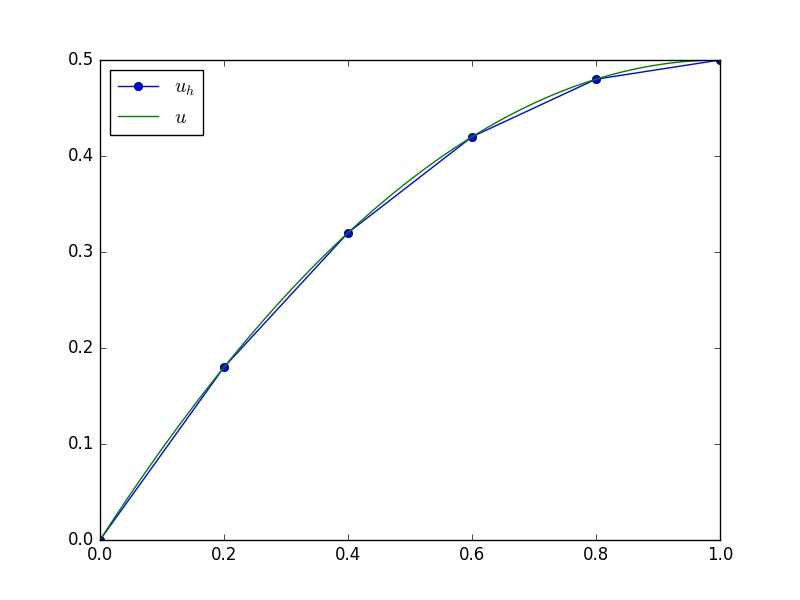
\includegraphics[width=0.8\textwidth]{./cap_mef1d/dados/ex_cc_n/ex_cc_n}
%   \caption{Esboço dos gráficos das soluções referentes ao Exemplo \ref{ex:cc_n}.}
%   \label{fig:ex_cc_n}
% \end{figure}

\begin{lstlisting}[caption=ex\_mef1d\_neumann.py]
from mpi4py import MPI

# malha
from dolfinx import mesh
domain = mesh.create_unit_interval(MPI.COMM_WORLD,
                                   nx = 5)
# espaço
from dolfinx import fem
V = fem.functionspace(domain, ('P', 1))

# c.c. dirichlet
import numpy as np
from dolfinx.fem import dirichletbc, locate_dofs_geometrical
uD = fem.Function(V)
uD.interpolate(lambda x: np.full(x.shape[1], 0.))

def boundary_D(x):
    return np.isclose(x[0], 0.)

dofs_D = locate_dofs_geometrical(V, boundary_D)
bc = dirichletbc(uD, dofs_D)

# problema mef
import ufl
from dolfinx import default_scalar_type
from dolfinx.fem.petsc import LinearProblem
u = ufl.TrialFunction(V)
v = ufl.TestFunction(V)

f = fem.Constant(domain, default_scalar_type(1.))

a = ufl.dot(ufl.grad(u), ufl.grad(v)) * ufl.dx
L = f * v * ufl.dx

problem = LinearProblem(a, L, bcs=[bc])
uh = problem.solve()

# armazena para visualização (paraview)
from dolfinx import io
from pathlib import Path
results_folder = Path("results")
results_folder.mkdir(exist_ok=True, parents=True)
filename = results_folder / "u"
with io.XDMFFile(domain.comm, filename.with_suffix(".xdmf"), "w") as xdmf:
    xdmf.write_mesh(domain)
    xdmf.write_function(uh)

\end{lstlisting}

\end{ex}

Agora, consideramos o seguinte problema com condições de Neumann não-homogênea em $x=L$: encontrar $u$ tal que
\begin{align}
  &-u'' = f,\quad \forall x\in I=[0, L],\label{eq:cc_n2_eq}\\
  &u(0) = u_0,\quad u'(L) = \alpha,\label{eq:cc_n2_bc}
\end{align}
com $u_0$, $\alpha$ e $f$ dados.

Tomando uma função teste $v\in V:=\{v\in H^1(I);~v(0)=0\}$ e multiplicando-a em \eqref{eq:cc_n2_eq}, obtemos
\begin{equation}
  - \int_I u''v\,dx = \int_I fv\,dx.
\end{equation}
Aplicando a integração por partes, temos
\begin{equation}
  \int_I u'v'\,dx - \alpha v(L)= \int_I fc\,dx.
\end{equation}
Desta forma, definimos o seguinte problema fraco associado: encontrar $u\in \tilde{V} := \{v\in H^1(I);~v(0)=u_0\}$ tal que
\begin{align}
  a(u,v) - b( = L(v),\quad\forall v\in V,
\end{align}
onde $a(u,v)$ é a forma bilinear
\begin{equation}
  a(u,v) = \int_I u'v'\,dx
\end{equation}
e $L(v)$ é a forma linear
\begin{equation}
  L(v) = \int_I fv\,dx + \alpha v(L).
\end{equation}

\begin{ex}\label{ex:cc_n2}
  Consideramos o problema
  \begin{align}
    &-u'' = 1,\quad x\in I=[0,1],\label{eq:ex_cc_n2_eq}\\
    &u(0) = 0,\quad u'(1) = 1.\label{eq:ex_cc_n2_bc}
  \end{align}
Sua solução analítica é $u(x) = -x^2/2+2x$. 

Agora, consideramos o seguinte problema fraco associado: encontrar $u\in V=\{v\in H^1(I);~v(0)=0\}$ tal que
\begin{equation}
  a(u,v) = L(v),\quad\forall v\in V,
\end{equation}
com
\begin{equation}
  a(u, v) = \int_I u'v'\,dx
\end{equation}
e
\begin{equation}
  L(v) = \int_I fv\,dx + 1\cdot v(1).
\end{equation}

Então, consideramos o seguinte problema de elementos finitos associado: encontrar $u_h\in V_h = \{v_h\in P_1(I);~v_h(0)=0\}$ tal que
\begin{equation}
  a(u_h, v_h) = L(v_h),\quad\forall v_h\in V_h.
\end{equation}

% A Figura \ref{fig:ex_cc_n2} apresenta o esboço dos gráficos da solução analítica $u$ e da sua aproximação de elementos finitos $u_h$, esta construída no espaço dos polinômios lineares por partes sobre uma malha uniforme de $5$ células.

% \begin{figure}[h!]
%   \centering
%   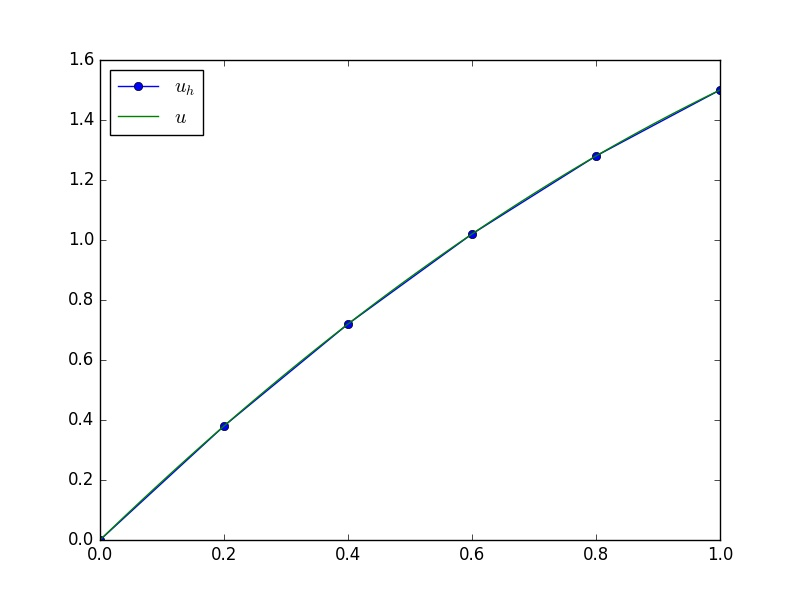
\includegraphics[width=0.8\textwidth]{./cap_mef1d/dados/ex_cc_n2/ex_cc_n2}
%   \caption{Esboço dos gráficos das soluções referentes ao Exemplo \ref{ex:cc_n2}.}
%   \label{fig:ex_cc_n2}
% \end{figure}

\begin{lstlisting}[caption=ex\_mef1d\_neumann\_nh.py]
from mpi4py import MPI

# malha
from dolfinx import mesh
domain = mesh.create_unit_interval(MPI.COMM_WORLD,
                                   nx = 5)
# espaço
from dolfinx import fem
V = fem.functionspace(domain, ('P', 1))

# c.c. dirichlet
import numpy as np
from dolfinx.fem import dirichletbc, locate_dofs_geometrical
uD = fem.Function(V)
uD.interpolate(lambda x: np.full(x.shape[1], 0.))

def boundary_D(x):
    return np.isclose(x[0], 0.)

dofs_D = locate_dofs_geometrical(V, boundary_D)
bc = dirichletbc(uD, dofs_D)

# problema mef
import ufl
from dolfinx import default_scalar_type
from dolfinx.fem.petsc import LinearProblem
u = ufl.TrialFunction(V)
v = ufl.TestFunction(V)

f = fem.Constant(domain, default_scalar_type(1.))
g = fem.Constant(domain, default_scalar_type(1.))

a = ufl.dot(ufl.grad(u), ufl.grad(v)) * ufl.dx
L = f * v * ufl.dx
L += g * v * ufl.ds

problem = LinearProblem(a, L, bcs=[bc])
uh = problem.solve()

# armazena para visualização (paraview)
from dolfinx import io
from pathlib import Path
results_folder = Path("results")
results_folder.mkdir(exist_ok=True, parents=True)
filename = results_folder / "u"
with io.XDMFFile(domain.comm, filename.with_suffix(".xdmf"), "w") as xdmf:
    xdmf.write_mesh(domain)
    xdmf.write_function(uh)
\end{lstlisting}

\end{ex} 

\subsection{Condições de Robin}
\badgeRevisar

Consideramos o seguinte problema com condições de contorno de Robin{\robin}: encontrar $u$ tal que
\begin{align}
  &-u'' = f,\quad \forall x\in I=[0, L],\label{eq:cc_r_eq}\\
  &u'(0) = r_0(u(0)-s_0),~ -u'(L) = r_L(u(L)-s_L),\label{eq:cc_r_bc}
\end{align}
com $r_0$, $r_L$, $s_0$, $s_L$ e $f$ dados.

Tomando uma função teste $v\in V= H^1(I)$ e multiplicando-a em \eqref{eq:cc_r_eq}, obtemos
\begin{equation}
  - \int_I u''v\,dx = \int_I fv\,dx.
\end{equation}
Aplicando a integração por partes, temos
\begin{equation}
  \int_I u'v'\,dx - \underbrace{u'(L)v(L)}_{-u'(L)=r_L(u(L)-s_L)} + \underbrace{u'(0)v(0)}_{u'(0)=r_0(u(0)-s_0)} = \int_I fc\,dx.
\end{equation}
ou, mais adequadamente,
\begin{equation}
  \int_I u'v'\,dx + r_Lu(L)v(L) +r_0u(0)v(0) = \int_I fc\,dx + r_Ls_Lv(L) + r_0s_0v(0).
\end{equation}
Desta forma, definimos o seguinte problema fraco associado: encontrar $u\in H^1(I)$ tal que
\begin{align}
  a(u,v) = L(v),\quad\forall v\in V,
\end{align}
onde $a(u,v)$ é a forma bilinear
\begin{equation}
  a(u,v) = \int_I u'v'\,dx + r_Lu(L)v(L) + r_0u(0)v(0)
\end{equation}
e $L(v)$ é a forma linear
\begin{equation}
  L(v) = \int_I fv\,dx + r_Ls_Lv(L) + r_0s_0v(0).
\end{equation}

\begin{ex}\label{ex:cc_r}
  Consideramos o problema
  \begin{align}
    &-u'' = 1,\quad x\in I=[0,1],\label{eq:ex_cc_r_eq}\\
    &u'(0) = u(0),\quad -u'(1) = u(1) - 1.\label{eq:ex_cc_r_bc}
  \end{align}
Sua solução analítica é $u(x) = -x^2/2+5x/6+5/6$. 

Aqui, tomamos o seguinte problema fraco: encontrar $u\in V=H^1(I)$ tal que
\begin{equation}
  a(u, v) = L(v),\quad\forall v\in V,
\end{equation}
onde
\begin{equation}
  a(u, v) = \int_I u'v'\,dx + u(1)v(1) + u(0)v(0)
\end{equation}
e
\begin{equation}
  L(v) = \int_I fv\,dx + 1\cdot v(1).
\end{equation}

Então, uma aproximação por elementos finitos lineares por partes pode ser obtida resolvendo o seguinte problema: encontrar $u_h\in V_h=P_1(I)$ tal que
\begin{equation}
  a(u_h, v_h) = L(v_h),\quad\forall v_h\in V_h.
\end{equation}

% A Figura \ref{fig:ex_cc_r} apresenta o esboço dos gráficos da solução analítica $u$ e da sua aproximação de elementos finitos $u_h$, esta construída no espaço dos polinômios lineares por partes sobre uma malha uniforme de $5$ células.

% \begin{figure}[h!]
%   \centering
%   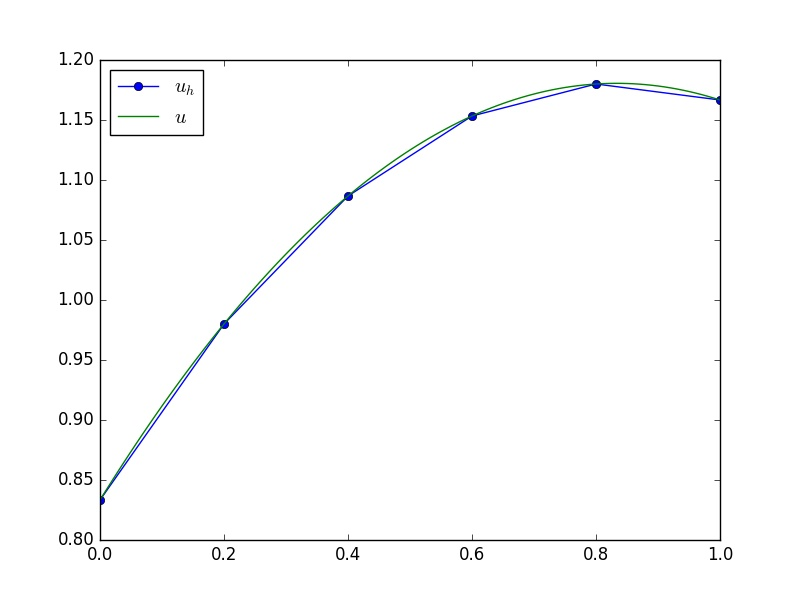
\includegraphics[width=0.8\textwidth]{./cap_mef1d/dados/ex_cc_r/ex_cc_r}
%   \caption{Esboço dos gráficos das soluções referentes ao Exemplo \ref{ex:cc_r}.}
%   \label{fig:ex_cc_r}
% \end{figure}

\begin{lstlisting}
from mpi4py import MPI

# malha
from dolfinx import mesh
domain = mesh.create_unit_interval(MPI.COMM_WORLD,
                                  nx = 5)
# espaço
from dolfinx import fem
V = fem.functionspace(domain, ('P', 1))

# boundary colors
from dolfinx.mesh import locate_entities
from dolfinx.mesh import meshtags
boundaries = [(0, lambda x: np.isclose(x[0], 0.)),
              (1, lambda x: np.isclose(x[0], 1.))]
facet_indices, facet_markers = [], []
fdim = domain.topology.dim - 1
for (marker, locator) in boundaries:
    facets = locate_entities(domain, fdim, locator)
    facet_indices.append(facets)
    facet_markers.append(np.full_like(facets, marker))
facet_indices = np.hstack(facet_indices).astype(np.int32)
facet_markers = np.hstack(facet_markers).astype(np.int32)
sorted_facets = np.argsort(facet_indices)
facet_tag = meshtags(domain, fdim, facet_indices[sorted_facets], facet_markers[sorted_facets])

# problema mef
import ufl
from dolfinx import default_scalar_type
from dolfinx.fem.petsc import LinearProblem
u = ufl.TrialFunction(V)
v = ufl.TestFunction(V)

f = fem.Constant(domain, default_scalar_type(1.))
g = fem.Constant(domain, default_scalar_type(1.))

ds = ufl.Measure('ds', domain=domain, subdomain_data=facet_tag)

a = ufl.dot(ufl.grad(u), ufl.grad(v)) * ufl.dx
a += u * v * ds(1) + u * v * ds(0)
L = f * v * ufl.dx
L += g * v * ds(1)

problem = LinearProblem(a, L, bcs=[])
uh = problem.solve()

# armazena para visualização (paraview)
from dolfinx import io
from pathlib import Path
results_folder = Path("results")
results_folder.mkdir(exist_ok=True, parents=True)
filename = results_folder / "u"
with io.XDMFFile(domain.comm, filename.with_suffix(".xdmf"), "w") as xdmf:
    xdmf.write_mesh(domain)
    xdmf.write_function(uh)  
\end{lstlisting}

\end{ex}

\subsection{Exercícios}
\badgeRevisar

\begin{exer}\label{exer:dcr}
  Considere o problema
  \begin{align}
    &-u'' + u' + 2u = -\cos(x),\quad x\in (0, \pi/2),\\
    &u(0)=-0,3,\quad u(\pi/2)=-0,1.
  \end{align}
  Obtenha uma aproximação por elementos finitos para a solução deste problema, empregando o espaço de elementos finitos linear sobre uma malha uniforme com $10$ células. Então, compare a aproximação computada com sua solução analítica $u(x) = 0,1(\sen(x)+3\cos(x))$, bem como, compute o erro $\|u-u_h\|_{L^2}$.
\end{exer}
\begin{resp}
  \ifispython
  \href{https://github.com/phkonzen/notas/blob/master/src/MetodoElementosFinitos/cap_mef1d/dados/exer_dcr/exer_dcr.py}{Código}.
  \fi
\end{resp}

\section{Malhas Auto-Adaptativas}\label{cap_mef1d_sec_adapt}
\badgeRevisar

Retornemos ao problema modelo \eqref{eq:prob_eq}-\eqref{eq:prob_bc}
\begin{align}
  -u'' &= f,\quad x\in I=[0,L],\\
  u(0) &= u(L) = 0.
\end{align}
A estimativa \textit{a posteriori} dada no Teorema \ref{teo:fem_est_a_posteriori}, indica que os elementos residuais $\eta_i(u_h)$ podem ser utilizados para estimarmos a precisão da aproximação por elementos finitos. Ou seja, espera-se que quanto menores forem os elementos residuais, mais precisa é a solução por elementos finitos. Além disso, como
\begin{equation}
  \eta_i(u_h) = h_i\|f - u_h''\|_{L^2(I_i)},
\end{equation}
podemos reduzir $\eta_i(u_h)$ diminuindo o tamanho da célula $I_i$.

Do observado acima, motiva-se o seguinte algoritmo de elementos finitos com refinamento automático de malha:
\begin{enumerate}
\item Escolhemos uma malha inicial.
\item Iteramos:
  \begin{enumerate}[2.]
  \item Resolvemos o problema de elementos finitos na malha corrente.
  \item Computamos $\eta_i(u_h)$ em cada célula da malha corrente.
  \item Com base na malha corrente, Contruímos uma nova malha pelo refinamento das células com os maiores valores de $\eta_i(u_h)$.
  \item Verificamos o critério de parada.
  \end{enumerate}
\end{enumerate}

Uma estratégia clássica para a escolha das células a serem refinadas é a seguinte: refina-se a $i$-ésima célula se
\begin{equation}\label{eq:ref_estrategia}
  \eta_i(u_h) > \alpha \max_{j=1, 2, \dotsc, n} \eta_j(u_h),
\end{equation}
onde escolhemos $0 < \alpha < 1$.

\begin{ex}\label{ex:modelo_adapt}
  Consideramos o problema
  \begin{align}
    -u'' &= e^{-100|x-\frac{1}{2}|},\quad x\in I=[0,1],\\
    u(0) &= u(1) = 0.
  \end{align}
  Aqui, computamos aproximações de elementos finitos no espaço das funções lineares por partes $V_{h,0} = \{v\in P_1(I);~v(0)=v(1)=0\}$ com sucessivos refinamentos de malha. Utilizamos uma malha inicial uniforme com 10 células e fazemos, então, 5 refinamentos sucessivos utilizando como critério de refinamento a estratégia \eqref{eq:ref_estrategia} com $\alpha = 0,5$. A Figura \ref{fig:ex_modelo_adapt} apresenta o esboço do gráfico da solução de elementos finitos na malha mais refinada. Além disso, na Tabela \ref{tab:ex_modelo_adapt} temos os o número de células e o $\eta_i(u_h)$ máximo respectivo.

\begin{figure}[h!]
  \centering
  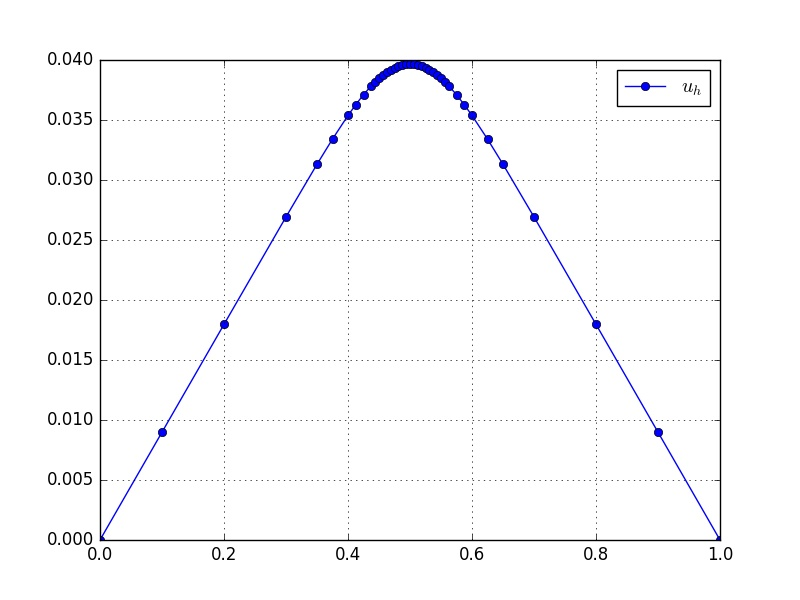
\includegraphics[width=0.8\textwidth]{./cap_mef1d/dados/ex_modelo_adapt/ex_modelo_adapt}
  \caption{Esboço dos gráficos das soluções referentes ao Exemplo \ref{ex:modelo_adapt}.}
  \label{fig:ex_modelo_adapt}
\end{figure}

\begin{table}[h!]
  \centering
  \begin{tabular}{lrc}
    \#malha & \#células & $\max_i\eta_i(u_h)$\\\hline
    0 & 10 & 5.0E-03\\
    1 & 12 & 2.0E-03\\
    2 & 14 & 8.6E-04\\
    3 & 22 & 2.9E-04\\
    4 & 30 & 1.4E-04\\
    5 & 38 & 6.1E-05\\\hline
  \end{tabular}
  \caption{Resultados referente ao Exemplo \ref{ex:modelo_adapt}.}
  \label{tab:ex_modelo_adapt}
\end{table}

\ifispython
Com o \fenics, a computação do problema de elementos finitos pode ser feita com o seguinte \href{https://github.com/phkonzen/notas/blob/master/src/MetodoElementosFinitos/cap_mef1d/dados/ex_modelo_adapt/ex_modelo_adapt.py}{código}:
\verbatiminput{./cap_mef1d/dados/ex_modelo_adapt/ex_modelo_adapt.py}
\fi
\end{ex}

\subsection{Exercícios}
\badgeRevisar

\begin{exer}\label{exer:modelo_refglobal}
  Use uma estratégia de sucessivos refinamentos globais para resolver o problema dado no Exemplo \ref{ex:modelo_adapt}. Compare seus resultados com aqueles obtidos no exemplo.
\end{exer}
\begin{resp}
  \ifispython
  \href{https://github.com/phkonzen/notas/blob/master/src/MetodoElementosFinitos/cap_mef1d/dados/exer_dcr/exer_dcr.py}{Código}.
  \fi  
\end{resp}

\section{Aplicação: EDP Evolutiva}\label{cap_mef1d_sec_calor}
\badgeConstrucao

Como exemplo de \hlemph{aplicação do método de elementos finitos (MEF) na solução de equações diferenciais parciais evolutivas no tempo}, consideramos a \hlemph{equação do calor} com dadas condição inicial e condições de contorno de Dirichlet homogêneas
\begin{subequations}\label{cap_mef1d_sec_calor:eq:prob}
  \begin{align}
    &u_t = \alpha u_{xx} + f, ~(t,x)\in (0, t_f]\times (a, b),\\
    &u(0, x) = u_0(x), x\in [a, b],\\
    &u(t, a) = u(t, b) = 0, ~t\in [0, t_f],
  \end{align}
\end{subequations}
onde $f = f(t, x)$ denota uma dada fonte.

\subsection{Discretização do Tempo}

Consideramos os $n_t+1$ tempos discretos $t^{(k)} = k h_t$, passo no tempo $h_t = t_f/n_t$, $k = 0, 1, 2, \dotsc, n_t$. Seguindo esquema $\theta$ denotando $u^{(k)} \approx u\left(t^{(k)}, x\right)$ e $f^{(k)} = f\left(t^{(k)}, x\right)$, o problema \eqref{cap_mef1d_sec_calor:eq:prob} pode ser aproximado pela iteração
\begin{subequations}\label{cap_mef1d_sec_calor:eq:theta}
  \begin{align}
    &\frac{u^{(k+1)} - u^{(k)}}{h_t} = \theta \left(\alpha u^{(k+1)}_{xx} + f^{(k+1)}\right)\nonumber\\
    &\qquad\qquad\qquad\;\; (1-\theta) \left(\alpha u^{(k)}_{xx} + f^{(k)}\right),\\
    &u^{(k+1)}(a) = u^{(k+1)}(b) = 0,
  \end{align}
\end{subequations}
onde $u^{(0)} = u_0$. 

\begin{obs}\normalfont{(Esquema $\theta$.)}
  O esquema $\theta$ e um forma robusta de escrever diferentes esquemas de discretização em uma única expressão:
  \begin{itemize}
    \item $\theta = 0.$: Euler explícito.
    \item $\theta = 1.$: Euler implícito.
    \item $\theta = 0.5$: Crank-Nicolson.
  \end{itemize}
\end{obs}

Por simplificação da notação, vamos suprimir o super-índice $k$, denotando $u^{(k+1)} := u$, $u^{(k)} = u^0$ e similar para $f^{(k)}$. Com isso e rearranjando os termos, cada iteração \eqref{cap_mef1d_sec_calor:eq:theta} se resume ao seguinte problema de valores de contorno
\begin{subequations}\label{cap_mef1d_sec_calor:eq:theta-iter}
  \begin{align}
    &-\alpha\theta u_{xx} + \frac{1}{h_t}u = \frac{1}{h_t}u^0 + (1-\theta)\alpha u^0_{xx} \nonumber\\
    &\qquad\qquad\qquad\quad + (1-\theta)f^0 + \theta f,\\
    &u(a) = u(b) = 0.
  \end{align}
\end{subequations}

\subsection{Formulação de Elementos Finitos}

A formulação fraca do problema \eqref{cap_mef1d_sec_calor:eq:theta-iter} consiste em: encontrar $u\in V := H^1_0(a, b)$ tal que
\begin{equation}
  a(u, v) = L(v), ~\forall v\in V,
\end{equation}
onde
\begin{align}
  &a(u, v) := \int_a^b \theta\alpha u'v'\,dx + \int_a^b \frac{1}{h_t}uv\,dx,\\
  &L(v) := (1-\theta)\int_a^b \alpha u^{0'}v'\,dx + \int_a^b \frac{1}{h_t}u^0v\,dx\nonumber\\
  &\qquad \theta\int_a^b fv\,dx + (1-\theta)\int_a^b f^0v\,dx
\end{align}

Então, assumindo uma malha com $n_x$ células $I_i = [x_i, x_{i+1}]$ de tamanho $h_x = (b-a)/n_x$ e nodos $x_i = a + (i-1)h_x$, $i = 0, 1, 2, \dotsc, n_x$, escolhemos o espaço de elementos finitos
\begin{equation}
  V_{h,0} := \{v\in C^0([a,b]): ~v|_{I_i}\in P_1(I_i), ~i=0,1,\dotsc,n_x, v(a)=v(b)=0\}.
\end{equation}
Com isso, a formulação de elementos finitos do problema \eqref{cap_mef1d_sec_calor:eq:theta-iter} consiste em: encontrar $u_h\in V_{h,0}$ tal que
\begin{equation}
  a(u_h, v_h) = L(v_h), ~\forall v_h\in V_{h,0}.
\end{equation}

\begin{ex}
  Consideramos o seguinte problema de calor
  \begin{subequations}
    \begin{align}
      &u_t = u_{xx} + (\pi^2-1)e^{-t}\sen(\pi x), ~(t,x)\in (0,1]\times (0,1),\\
      &u(0,x) = \sen(\pi x), ~x\in [0, 1],\\
      &u(t,0) = u(t,1) = 0.
    \end{align}
  \end{subequations}

\begin{lstlisting}
from mpi4py import MPI
import ufl
from dolfinx import mesh
from dolfinx import fem
from dolfinx import default_scalar_type
from dolfinx.fem.petsc import LinearProblem

# parâmetros
tf = 1.
alpha = 1.

# esquema theta
theta = 0.5

# discretização no tempo
nt = 10
ht = tf/nt

# malha
domain = mesh.create_unit_interval(MPI.COMM_WORLD,
                                    nx = 5)
x = ufl.SpatialCoordinate(domain)

# espaço
V = fem.functionspace(domain, ('P', 1))

# fonte
f = fem.Function(V)
def f(t,x):
    return (ufl.pi**2-1.)*ufl.exp(-t)*ufl.sin(ufl.pi*x[0])

# condição de contorno
import numpy as np
uD = fem.Function(V)
uD.interpolate(lambda x: np.full(x.shape[1], 0.))

def boundary_D(x):
    return np.logical_or(np.isclose(x[0], 0.),
                          np.isclose(x[0], 1.))

dofs_D = fem.locate_dofs_geometrical(V, boundary_D)
bc = fem.dirichletbc(uD, dofs_D)

# mef fun.s
u = ufl.TrialFunction(V)
v = ufl.TestFunction(V)

# condição inicial
t = 0.
u0 = fem.Function(V)
u0.interpolate(lambda x: np.sin(np.pi*x[0]))

# fonte
def f(t, x):
    return (ufl.pi**2-1.)*ufl.exp(-t)*ufl.sin(ufl.pi*x[0])

# visualização (paraview)
from dolfinx import io
from pathlib import Path
results_folder = Path("results")
results_folder.mkdir(exist_ok=True, parents=True)

# iteração no tempo
for k in range(nt):
    t += ht

    # forma bilinear
    a = theta * ufl.dot(ufl.grad(u), ufl.grad(v)) * ufl.dx
    a += u * v / ht * ufl.dx

    # forma linear
    L = (theta-1.) * ufl.dot(ufl.grad(u0), ufl.grad(v)) * ufl.dx
    L += u0 * v / ht * ufl.dx
    L += theta * f(t, x) * v * ufl.dx
    L += (1.-theta) * f(t-ht, x) * v * ufl.dx

    problem = LinearProblem(a, L, bcs=[bc])
    uh = problem.solve()

    # armazena para visualização (paraview)
    filename = results_folder / f"u_{k:0>6}"
    with io.XDMFFile(domain.comm, filename.with_suffix(".xdmf"), "w") as xdmf:
        xdmf.write_mesh(domain)
        xdmf.write_function(uh, t)

    u0.x.array[:] = uh.x.array[:]  
\end{lstlisting}
\end{ex}


\subsection{Exercícios}
\badgeConstrucao

\section{Aplicação: EDP de Advecção-Difusão}\label{cap_mef1d_sec_eqad}
\badgeConstrucao

\subsection{Exercícios}
\badgeConstrucao


\section{Aplicação: EDP Não-Linear}\label{cap_mef1d_sec_eqnl}
\badgeConstrucao

Como exemplo de aplicação do MEF na solução de \hlemph{equações diferenciais parciais não-lineares}, consideramos a \hlemph{equação de Fisher}{\fisher} com dadas condição inicial e condições de contorno de Neumann{\neumann}
\begin{subequations}\label{cap_mef1d_sec_eqnl:eq:prob}
  \begin{align}
    &u_t = u_{xx} + u(1-u), ~(t,x)\in (0,t_f]\times (0,1),\\
    &u(0, x) = u_0(x), ~x\in [0,1],\\
    &u_x(t,0) = u_x(t,1) = 0, ~t\in [0,t_f].
  \end{align}
\end{subequations}

\subsection{Discretização do Tempo}

Consideramos os $n_t+1$ tempos discretos $t^{(k)} = k h_t$, passo no tempo $h_t = t_f/n_t$, $k = 0, 1, 2, \dotsc, n_t$. Seguindo esquema $\theta$ denotando $u^{(k)} \approx u\left(t^{(k)}, x\right)$, o problema \eqref{cap_mef1d_sec_eqnl:eq:prob} pode ser aproximado pela iteração
\begin{subequations}\label{cap_mef1d_sec_eqnl:eq:theta}
  \begin{align}
    &\frac{u^{(k+1)} - u^{(k)}}{h_t} = \theta \left[u^{(k+1)}_{xx} + u^{(k+1)}\left(1-u^{(k+1})\right)\right]\nonumber\\
    &\qquad\qquad\qquad\;\; (1-\theta) \left[u^{(k)}_{xx} + + u^{(k)}\left(1-u^{(k)}\right)\right],\\
    &u_x^{(k+1)}(0) = u_x^{(k+1)}(1) = 0,
  \end{align}
\end{subequations}
onde $u^{(0)} = u_0$. 

\begin{obs}\normalfont{(Esquema $\theta$.)}
  O esquema $\theta$ e um forma robusta de escrever diferentes esquemas de discretização em uma única expressão:
  \begin{itemize}
    \item $\theta = 0.$: Euler explícito.
    \item $\theta = 1.$: Euler implícito.
    \item $\theta = 0.5$: Crank-Nicolson.
  \end{itemize}
\end{obs}

Por simplificação da notação, vamos suprimir o super-índice $k$, denotando $u^{(k+1)} := u$, $u^{(k)} = u^0$. Com isso e rearranjando os termos, cada iteração \eqref{cap_mef1d_sec_eqnl:eq:theta} se resume ao seguinte problema de valores de contorno
\begin{subequations}\label{cap_mef1d_sec_eqnl:eq:theta-iter}
  \begin{align}
    &\frac{1}{h_t}u - \frac{1}{h_t}u^0 - \theta\left[u_xx + u(1-u)\right]\nonumber\\
    &\qquad\qquad - (1-\theta)\left[u^0_xx + u^0(1-u^0)\right],\\
    &u_x(0) = u_x(1) = 0.
  \end{align}
\end{subequations}

\subsection{Formulação de Elementos Finitos}
\badgeRevisar

A formulação fraca do problema \eqref{cap_mef1d_sec_eqnl:eq:theta-iter} consiste em: encontrar $u\in V := H^1[0,1]$ tal que
\begin{equation}
  F(u;v) = 0, ~\forall v\in V,
\end{equation}
onde
\begin{equation}
  \begin{aligned}
    & F(u; v) := \int_0^1 \frac{1}{h_t}u\,dx - \int_0^1 \frac{1}{h_t}u^0\,dx\\
    &\qquad + \theta\int_0^1 u_xv_x\,dx - \theta\int_0^1 u(1-u)v\,dx\\
    &\qquad + (1-\theta)\int_0^1 u^0_x v_x\,dx - (1-\theta)\int_0^1 u^0(1-u^0)v\,dx.
  \end{aligned}
\end{equation}

Então, assumindo uma malha com $n_x$ células $I_i = [x_i, x_{i+1}]$ de tamanho $h_x = 1/n_x$ e nodos $x_i = (i-1)h_x$, $i = 0, 1, 2, \dotsc, n_x$, escolhemos o espaço de elementos finitos
\begin{equation}
  V_h := \{v\in C^0([a,b]): ~v|_{I_i}\in P_1(I_i), ~i=0,1,\dotsc,n_x\}.
\end{equation}
Com isso, a formulação de elementos finitos do problema \eqref{cap_mef1d_sec_eqnl:eq:theta-iter} consiste em: encontrar $u_h\in V_h$ tal que
\begin{equation}\label{cap_mp_sec_eqnl:eq:fem}
  F(u_h; v) = 0, ~\forall v_h\in V_h.
\end{equation}

\begin{obs}
  O problema \eqref{cap_mp_sec_eqnl:eq:fem} consiste em um sistema de equações não-lineares.
\end{obs}

\begin{ex}
  Consideramos a equação de Fisher com condições inicial e de contorno
  \begin{subequations}
    \begin{align}
      &u_t = u_{xx} + u(1-u), ~t\in(0,t_f)\times(0,1),\\
      &u(0,x) = \cos^2(\pi x), ~x\in[0,1],\\
      &u_x(t,0)=u_x(t,1)=0, ~t\in[0,t_f],
    \end{align}
  \end{subequations}
  com $tf=5$.

\begin{lstlisting}[caption=ex\_mef1d\_fisher.py]
  from mpi4py import MPI
  import numpy as np
  import ufl
  from dolfinx import mesh
  from dolfinx import fem
  from dolfinx import default_scalar_type
  from dolfinx.fem.petsc import NonlinearProblem
  from dolfinx.nls.petsc import NewtonSolver
  
  # parâmetros
  tf = 5.
  
  # esquema theta
  theta = 0.5
  
  # discretização no tempo
  nt = 100
  ht = tf/nt
  
  # malha
  domain = mesh.create_unit_interval(MPI.COMM_WORLD,
                                     nx = 5)
  x = ufl.SpatialCoordinate(domain)
  
  # espaço
  V = fem.functionspace(domain, ('P', 1))
  
  # mef fun.s
  v = ufl.TestFunction(V)
  u = fem.Function(V)
  
  # condição inicial
  t = 0.
  u0 = fem.Function(V)
  u0.interpolate(lambda x: np.cos(np.pi*x[0])**2)
  
  # inicialização
  u.x.array[:] = u0.x.array[:]
  
  # visualização (paraview)
  from dolfinx import io
  from pathlib import Path
  results_folder = Path("results")
  results_folder.mkdir(exist_ok=True, parents=True)
  
  # armazena para visualização (paraview)
  filename = results_folder / f"u_{0:0>6}"
  with io.XDMFFile(domain.comm, filename.with_suffix(".xdmf"), "w") as xdmf:
      xdmf.write_mesh(domain)
      xdmf.write_function(u, 0.)
  
  
  # iteração no tempo
  for k in range(nt):
      
      t += ht
      print(f"{k+1}: t = {t:.4g}")
  
      # forma fraca
      ## time term
      F = 1./ht * u * v * ufl.dx
      F -= 1./ht * u0 * v * ufl.dx
      ## diffusion term
      F += theta * ufl.dot(ufl.grad(u), ufl.grad(v)) * ufl.dx
      F += (1.-theta) * ufl.dot(ufl.grad(u0), ufl.grad(v)) * ufl.dx
      ## reaction term
      F -= theta * u * (1. - u) * v * ufl.dx
      F -= (1.-theta) * u0 * (1. - u0) * v * ufl.dx
  
      problem = NonlinearProblem(F, u)
      solver = NewtonSolver(MPI.COMM_WORLD, problem)
      n, converged = solver.solve(u)
      print(f"\tNewton iterations: {n}")
      assert(converged)
  
      # armazena para visualização (paraview)
      filename = results_folder / f"u_{k+1:0>6}"
      with io.XDMFFile(domain.comm, filename.with_suffix(".xdmf"), "w") as xdmf:
          xdmf.write_mesh(domain)
          xdmf.write_function(u, t)
  
      u0.x.array[:] = u.x.array[:]  
\end{lstlisting}
\end{ex}

\subsection{Exercícios}
\badgeConstrucao


\section{Seleção de Aplicações}\label{cap_mef1d_sec_aps}
\badgeRevisar

\subsection{Sistemas de Equações}
\badgeRevisar

Consideramos o seguinte problema de equações diferenciais ordinárias com valores de contorno
\begin{align}
  &-u_0'' + u_1 = f_0,\forall x\in (0, L)\\ 
  &-u_1'' + u_0 = f_1,\forall x\in (0, L)\\
  &u_0(0)=u_{00},\quad u_0(L)=u_{0L},\\
  &u_1(0)=u_{10},\quad u_1(L)=u_{1L},
\end{align}
onde $f_0$, $f_1$, $u_{00}$, $u_{0L}$, $u_{10}$, $u_{1L}$ são dados.

Para construirmos uma aproximação por elementos finitos podemos tomar o seguinte problema fraco associado: encontrar $u = (u_0, u_1)\in V_0\times V_1$ tal que
\begin{equation}
  a(u, v) = L(v), \forall v = (v_0, v_1)\in V\times V,
\end{equation}
onde $V_0 = \{v\in H^1(I);~v_0(0)=u_{00},~v_0(L)=u_{0L}\}$, $V_1=\{v_1\in H^1(I);~v_1(0)=u_{10},~v_1(L)=u_{1L}\}$, $V = \{v\in H^1(I);~v(0)=v(L)=0\}$, a forma bilinear é
\begin{equation}\label{eq:sis_lin_bilinear}
  a(u, v) = \int_{I} u_0'v_0'\,dx + \int_{I} u_1'v_1'\,dx + \int_{I} u_0v_0\,dx + \int_{I} u_1v_1\,dx
\end{equation}
e a forma linear é
\begin{equation}\label{eq:sis_lin_linear}
  L(v) = \int_I f_0v_0\,dx + \int_I f_1v_1\,dx.
\end{equation}

Então, o problema de elemento finitos associado no espaço das funções lineares por partes lê-se: encontrar $u_h = (u_{h0}, u_{h1})\in V_{h0}\times V_{h1}$ tal que
\begin{equation}
  a(u_h, v_h) = L(v_h), \forall v_h = (v_{h0}, v_{h1})\in V_h\times V_h,
\end{equation}
onde $V_{h0} = \{v_h\in P_1(I);~v_{h0}(0)=u_{00},~v_{h0}(L)=u_{0L}\}$, $V_{h1}=\{v_{h1}\in P_1(I);~v_{h1}(0)=u_{10},~v_{h1}(L)=u_{1L}\}$, $V_h = \{v_h\in P_1(I);~v_h(0)=v_h(L)=0\}$.

\begin{ex}\label{ex:sis_lin}
  Consideramos o seguinte problema de valor de contorno
\begin{align}
  &-u_0'' + u_1 = \sen(x)+\cos(x),\forall x\in (-\pi, \pi)\\ 
  &-u_1'' + u_0 = \cos(x)-\sin(x),\forall x\in (-\pi, \pi)\\
  &u_0(-\pi)=0,\quad u_0(\pi)=0,\\
  &u_1(-\pi)=-1,\quad u_1(\pi)=-1.
\end{align}
Considerando elementos lineares por partes, temos a seguinte formulação de elementos finitos: encontrar $u_h = (u_{h0}, u_{h1})\in V_{h0}\times V_{h1}$ tal que
\begin{equation}
  a(u_h, v_h) = L(v_h), \forall v_h = (v_{h0}, v_{h1})\in V_h\times V_h,
\end{equation}
onde $V_{h0} = \{v_h\in P_1(I);~v_{h0}(0)=v_{h0}(L)=0\}$, $V_{h1}=\{v_{h1}\in P_1(I);~v_{h1}(0)=v_{h1}(L)=-1\}$, $V_h = \{v_h\in P_1(I);~v_h(0)=v_h(L)=0\}$, com as formas bilinear e linear são dadas em \eqref{eq:sis_lin_bilinear} e \eqref{eq:sis_lin_linear}, respectivamente.

A Figura \ref{fig:ex_sis_lin} apresenta o esboço dos gráficos das soluções analíticas $u_0(x)=\sen(x)$ e $u_1(x)=\cos(x)$ e de suas aproximações de elementos finitos $u_{h0}$ e $u_{h1}$, estas construídas no espaço dos polinômios lineares por partes sobre uma malha uniforme de $5$ células.

\begin{figure}[h!]
  \centering
  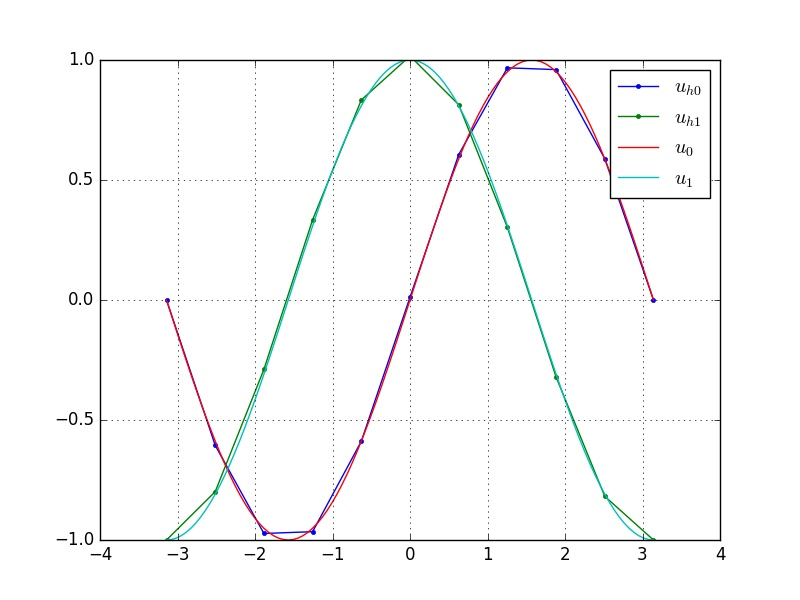
\includegraphics[width=0.8\textwidth]{./cap_mef1d/dados/ex_sis_lin/ex_sis_lin}
  \caption{Esboço dos gráficos das soluções referentes ao Exemplo \ref{ex:sis_lin}.}
  \label{fig:ex_sis_lin}
\end{figure}

\ifispython
Com o \fenics, a computação do problema de elementos finitos pode ser feita com o seguinte \href{https://github.com/phkonzen/notas/blob/master/src/MetodoElementosFinitos/cap_mef1d/dados/ex_sis_lin/ex_sis_lin.py}{código}:
\verbatiminput{./cap_mef1d/dados/ex_sis_lin/ex_sis_lin.py}
\fi
\end{ex}

\subsection{Exercícios}
[[tag:construcao]]


%Este trabalho está licenciado sob a Licença Atribuição-CompartilhaIgual 4.0 Internacional Creative Commons. Para visualizar uma cópia desta licença, visite http://creativecommons.org/licenses/by-sa/4.0/deed.pt_BR ou mande uma carta para Creative Commons, PO Box 1866, Mountain View, CA 94042, USA.

\chapter{Método de elementos finitos em 2D}\label{cap_mef2d}
\thispagestyle{fancy}

\section{Malha e espaço}\label{cap_mef2d_sec_malha}

\subsection{Malha}

Seja $\Omega\subset \mathbb{R}^2$ um domínio limitado com fronteira $\p\Omega$ suave e poligonal. Uma malha (ou triangularização) $\mathcal{K}$ de $\Omega$ é um conjunto de $\{K\}$ células (ou elementos) $K$, tal que $\Omega = \cup_{K\in\mathcal{K}}K$ e tal que a interseção de duas células é ou um lado, um canto ou vazio.

Classicamente as células $K$ são escolhidas como triângulos. O tamanho do lado de maior comprimento do triangulo $K$ define o chamado \emph{tamanho local da malha} $h_K$. O tamanho global da malha é definida por $h = \max_{K\in\mathcal{K}} h_K$.

Uma malha é dita \emph{regular} quando existe uma constante $c_0 > 0$ tal que $c_K > c_0$ para todo $K\in\mathcal{K}$, sendo $c_K := h_K/d_k$ e $d_K$ o diâmetro do circulo inscrito em $K$. Esta condição significa que os triângulo $K$ da malha não podem ter ângulos muito grandes nem muito pequenos. Ao longo do texto, a menos que especificado o contrário, assumiremos trabalhar com malhas regulares.

\subsection{Espaço dos polinômios lineares por partes}

Seja $K$ um triângulo e seja $P_1(K)$ o espaço das funções lineares em $K$, i.e.
\begin{equation}
  P_1(K) = \{v;~v=c_0+c_1x_1+c_2x+2,~(x_1,x_2)\in K,~c_0,c_1,c_2\in\mathbb{R}\}.
\end{equation}

Observemos que toda função $v\in P_1(K)$ é unicamente determinada por seus valores nodais $\alpha_i = v(N_i)$, $i=0, 1, 2$, onde $N_i = (x_1^{(i)}, x_2^{(i)})$ é o $i$-ésimo nodo (vértice) do triângulo $K$. Isto segue do fato de que
\begin{equation}
  \begin{bmatrix}
    1 & x_1^{(1)} & x_2^{(1)}\\
    1 & x_1^{(2)} & x_2^{(2)}\\
    1 & x_1^{(3)} & x_2^{(2)}
  \end{bmatrix}
  \begin{bmatrix}
    c_0\\
    c_1\\
    c_2
  \end{bmatrix} = 
  \begin{bmatrix}
    \alpha_1\\
    \alpha_2\\
    \alpha_3
  \end{bmatrix}
\end{equation}
Computando o valor absoluto do determinante da matriz de coeficientes, obtemos $2|K|$, onde $|K|$ denota a área de $K$, a qual é não nula.

Afim de usarmos os valores nodais como graus de liberdade (incógnitas), nós introduzimos a seguinte base nodal $\{\lambda_1, \lambda_2, \lambda_3\}$ com
\begin{equation}
  \lambda_j(N_i) = \left\{
    \begin{array}{ll}
      1 &, i=j,\\
      0 &, i\neq j
    \end{array}
\right.,~i,j=0,1,2.
\end{equation}
Com esta base, toda função $v\in P_1(K)$ pode ser escrita como
\begin{equation}
  v = \alpha_1\lambda_1 + \alpha_2\lambda_2 + \alpha_3\lambda_3,
\end{equation}
onde $\alpha_i = v(N_i)$.

\subsection{Espaço contínuo dos polinômios lineares por partes}

O espaço contínuo dos polinômios lineares por partes na malha $\mathcal{K}$ é definido por
\begin{equation}
  V_h = \{v;~v\in C^0(\Omega),~v|_K\in P_1(K),~\forall K\in\mathcal{K}\}.
\end{equation}

Observemos que toda função $v\in V_h$ é unicamente determinada por seus valores nodais $\{v(N_j)\}_{j=1}^{n_p}$, onde $n_p$ é número de nodos da malha $\mathcal{K}$. De fato, os valores nodais determinam uma única função em $P_1(K)$ para cada $K\in\mathcal{K}$ e, portanto, uma função em $V_h$ é unicamente determinada por seus valores nos nodos. Agora, consideremos dois triângulos $K_1$ e $K_2$ compartilhando um lado $E = K_1\cap K_2$. Sejam $v_1$ e $v_2$ os dois únicos polinômios em $v_1\in P_1(K_1)$ e $v_2\in P_2(K_2)$, respectivamente determinados pelos valores nodais em $K_1$ e $K_2$. Como $v_1$ e $v_2$ também são polinômios lineares em $E$ e seus valores coincidem nos nodos de $E$, temos $v_1 = v_2$. Portanto, concluímos que toda função $v\in V_h$ é unicamente determinada por seus valores nodais.

Afim de termos os valores nodais como graus de liberdade (incógnitas), definimos a base nodas $\{\phi_j\}_{j=1}^{n_p}\subset V_h$ tal que
\begin{equation}
  \varphi_j(N_i) = \left\{
    \begin{array}{ll}
      1 &, i=j\\
      0 &, i\neq j
    \end{array}
\right.,~i,j=0, 1, \dotsc, n_p-1.
\end{equation}
Notemos que cada função base $\phi_j$ é contínua, linear por partes e com suporte somente em um pequeno conjunto de triângulos que compartilham o nodo $N_j$. Além disso, todo a função $v\in V_h$ pode, então, ser escrita como
\begin{equation}
  v = \sum_{i=0}^{n_p-1}\alpha_i\varphi_i,
\end{equation}
onde $\alpha_i = v(N_i)$, $i=0, 1, \ldots, n_p$, são os valores nodais de $v$.

\begin{ex}\label{ex:malha}
  A Figura \ref{fig:ex_malha} mostra o esboço de uma malha triangular no domínio $D = [0, 1]\times [0, 1]$.

  \begin{figure}[h!]
    \centering
    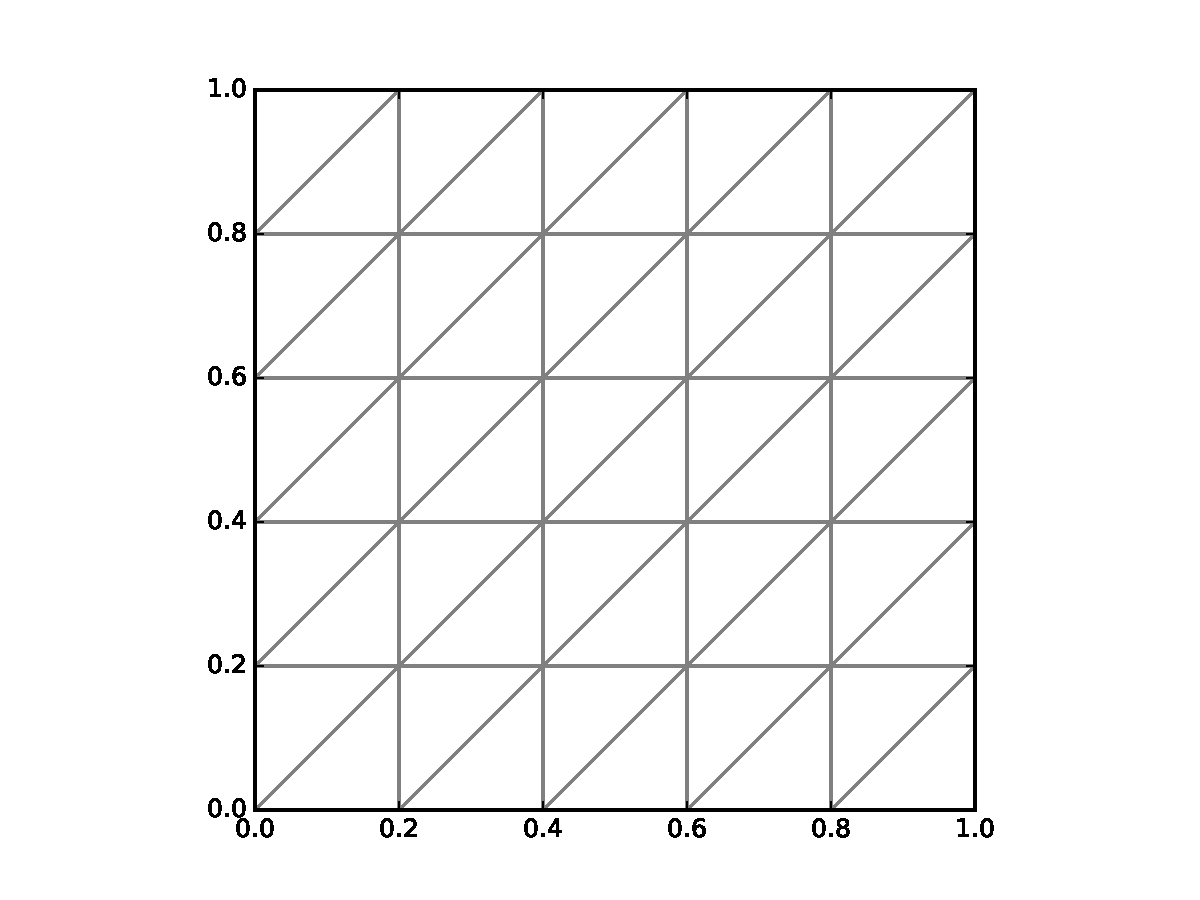
\includegraphics[width=0.7\textwidth]{./cap_mef2d/dados/ex_malha/fig_ex_malha}
    \caption{Esboço de uma malha triangular no domínio $D = [0, 1]\times [0, 1]$.}
    \label{fig:ex_malha}
  \end{figure}

\ifispython
Com o \fenics, podemos gerar esta malha com o seguinte \href{https://github.com/phkonzen/notas/blob/master/src/MetodoElementosFinitos/cap_mef2d/dados/ex_malha/ex_malha.py}{código}:
\verbatiminput{./cap_mef2d/dados/ex_malha/ex_malha.py}
\fi
\end{ex}

\section{Interpolação e projeção}\label{cap_mef2d_sec_interp}

\subsection{Interpolação}

Dada uma função contínua $f$ em um triângulo $K$ com nodos $N_i$, $i=0, 1, 2$, sua interpolação linear $\phi f \in P_1(K)$ é definida por
\begin{equation}
  \pi f = \sum_{i=0}^3 f(N_i)\varphi_i.
\end{equation}
Logo, temos $\pi f(N_i) = f(N_i)$ para todo $i=0, 1, 2$.

Afim de determinarmos estimativas para o erro de interpolação, precisamos da chamada derivada total de primeira ordem
\begin{equation}
  Df = \left(\left|\frac{\p f}{\p x_1}\right|^2 + \left|\frac{\p f}{\p x_2}\right|^2\right)^{1/2},
\end{equation}
e da derivada total de segunda ordem
\begin{equation}
  D^2f = \left(\left|\frac{\p^2 f}{\p x_1^2}\right|^2 + \left|\frac{\p^2 f}{\p x_1\p x_2}\right|^2 + \left|\frac{\p^2 f}{\p x_2^2}\right|^2\right)^{1/2}.
\end{equation}

\begin{prop}\normalfont{(Erro da interpolação no espaço linear)}\label{prop:interpl}
  A interpolação $\pi f$ satisfaz as seguintes estimativas
  \begin{align}
    \|f - \pi f\|_{L^2(K)} &\leq Ch_K^2\|D^2f\|_{L^2(K)},\label{eq:interpl_0}\\
    \|D(f - \pi f)\|_{L^2(K)} &\leq Ch_K\|D^2 f\|_{L^2(K)}.\label{eq:interpl_1}
  \end{align}
\end{prop}
\begin{dem}
  Veja \cite[Capítulo 4]{Brenner2008a}.
\end{dem}

\begin{obs}
  A constante $C$ dependo do inverso de $\sen(\theta_K)$ onde $\theta_K$ é o menor angulo de $K$. Desta forma, para um triângulo com $\theta_K$ muito pequeno, as estimativas \eqref{eq:interpl_0} e \eqref{eq:interpl_1} perdem sentido. Este fato indica a necessidade de se trabalhar com malhas regulares.
\end{obs}

A interpolação no espaço $V_h$ de uma dada função $f$ no domínio $\Omega$ é denotada também por $\pi f\in V_h$ e definida por
\begin{equation}
  \pi f = \sum_{i=0}^{n_p-1} f(N_i)\varphi_i.
\end{equation}

\begin{prop}\normalfont{(Erro da interpolação no espaço contínuo linear por partes)}\label{prop:interpc}
  O interpolador $\pi f\in V_h$ satisfaz as seguintes estimativas
  \begin{align}
    \|f - \pi f\|_{L^2(\Omega)}^2 &\leq C\sum_{K\in\mathcal{K}} h_K^4\|D^2 f\|_{L^2(K)}^2,\label{eq:interpc_0}\\
    \|D(f - \pi f)\|_{L^2(\Omega)}^2 &\leq C\sum_{K\in\mathcal{K}} h_K^2\|D^2 f\|_{L^2(K)}^2,\label{eq:interpc_1}.
  \end{align}
\end{prop}
\begin{dem}
  Demonstração análoga a Proposição \ref{prop:interp_linpartes}.
\end{dem}

\ifispython
\begin{ex}\label{ex:interp}
Consideremos a função $f(x_0,x_1) = \sen(\pi x_0)\cos(\pi x_1)$ definida no domínio $D = [0, 1]\times [0, 1]$. O seguinte \href{https://github.com/phkonzen/notas/blob/master/src/MetodoElementosFinitos/cap_mef2d/dados/ex_interp/ex_interp.py}{código} computa a interpolação de $f$ no espaço $V_h$ sobre uma malha triangular uniforme.

\verbatiminput{./cap_mef2d/dados/ex_interp/ex_interp.py}
\end{ex}
\fi

\subsection{Projeção $L^2$}

A projeto $L^2$ no espaço $V_h$ de uma dada uma função $f\in L^2(\Omega)$  é denotada por $P_hf\in V_h$ e definida por
\begin{equation}
  \int_\Omega (f-P_hf)v\,dx = 0,~\forall v\in V_h.
\end{equation}

Analogamente a projeção em uma dimensão (veja Subseção \ref{subsec:projecao_1d}), a projeção
\begin{equation}
  P_h f = \sum_{j=0}^{n_p-1} \xi_j\varphi_j,
\end{equation}
onde $\xi_j$ satisfaz o sistema linear
\begin{equation}
  M\pmb{\xi} = \pmb{b},
\end{equation}
onde $M = [m_{i,j}]_{i,j=0}^{n_p-1}$ é a matriz de massa com
\begin{equation}
  m_{i,j} = \int_{\Omega} \varphi_i\varphi_j\,dx
\end{equation}
e $\pmb{b} = (b_1,~b_2,~\dotsc,~b_{n_p-1})$ é o vetor de carga com
\begin{equation}
  b_i = \int_\Omega f\varphi_i\,dx.
\end{equation}

Também, vale o resultado análogo da melhor aproximação (veja \ref{teo:melhor_aprox}), i.e.
\begin{equation}
  \|f-P_hf\|_{L^2(\Omega)} \leq \|f - v\|_{L^2(\Omega)},\quad\forall v\in V_h.
\end{equation}
E, portanto, também temos a estimativa análoga para o erro de projeção (veja \ref{teo:erro_proj_1d})
\begin{equation}
  \|f-P_hf\|_{L^2(\Omega)}^2 \leq C\sum_{K\in\mathcal{K}} h_K^4\|D^2 f\|_{L^2(K)}^2.
\end{equation}
Tomando o tamanho global da malha, temos
\begin{equation}\label{eq:erro_projec_2d}
  \|f-P_hf\|_{L^2(\Omega)} \leq Ch^2\|D^2 f\|_{L^2(K)}.
\end{equation}

\ifispython
\begin{ex}\label{ex:projec}
Consideremos a função $f(x_0,x_1) = \sen(\pi x_0)\cos(\pi x_1)$ definida no domínio $D = [0, 1]\times [0, 1]$. O seguinte \href{https://github.com/phkonzen/notas/blob/master/src/MetodoElementosFinitos/cap_mef2d/dados/ex_projec/ex_projec.py}{código} computa a projeção de $f$ no espaço $V_h$ sobre uma malha triangular uniforme.

\verbatiminput{./cap_mef2d/dados/ex_projec/ex_projec.py}
\end{ex}
\fi

\subsection*{Exercícios}

\begin{exer}
  Verifique computacionalmente a Proposição \ref{prop:interpc} no caso da função $f(x_0,x_1) = \sen(\pi x_0)\cos(\pi x_1)$ interpolada sobre uma malha triangular uniforme sobre o domínio $D = [0, 1]\times [0, 1]$.
\end{exer}

\begin{exer}
  Verifique computacionalmente a estimativa \eqref{eq:erro_projec_2d} no caso da função $f(x_0,x_1) = \sen(\pi x_0)\cos(\pi x_1)$ projetada sobre uma malha triangular uniforme sobre o domínio $D = [0, 1]\times [0, 1]$.
\end{exer}

\section{Problema modelo}\label{cap_mef2d_sec_probmodelo}

Nesta seção, apresentaremos a aplicação do método de elementos finitos para a equação de Poisson\footnote{Siméon Denis Poisson, 1781 - 1840, matemático francês. Fonte: \href{https://en.wikipedia.org/wiki/Sim\%C3\%A9on_Denis_Poisson}{Wikipedia}.} com condições de Dirichlet\footnote{Johann Peter Gustav Lejeune Dirichlet, 1805 - 1859, matemático alemão. Fonte: \href{https://en.wikipedia.org/wiki/Peter_Gustav_Lejeune_Dirichlet}{Wikipedia}.}, i.e.: encontrar $u$ tal que
\begin{align}
  -\Delta u &= f,~x\in\Omega,\label{eq:mef2d_pm_eq}\\
  u &= 0,~x\in\p\Omega,\label{eq:mef2d_pm_bc}
\end{align}
onde $\Delta = \p^2/\p x_0^2 + \p^2/\p x_1^2$ é o operador de Laplace\footnote{Pierre-Simon, marquis de Laplace, 1749 - 1827, matemático francês. Fonte: \href{https://en.wikipedia.org/wiki/Pierre-Simon_Laplace}{Wikipedia}.} e $f$ é uma função dada.

\subsection{Formulação variacional}

A aplicação do método de elementos finitos é construída sobre a formulação fraca do problema \eqref{eq:mef2d_pm_eq}-\eqref{eq:mef2d_pm_bc}. Para obtermos esta, multiplicamos \eqref{eq:mef2d_pm_eq} por uma função teste $v$ em um espaço adequado $V_0$ e integramos no domínio $\Omega$, i.e.
\begin{equation}
  - \int_\Omega \Delta uv\,dx = \int_\Omega fv\,dx.
\end{equation}
Então, usando a fórmula de Green\footnote{George Green, 1793 - 1841, matemático britânico. Fonte: \href{https://en.wikipedia.org/wiki/George_Green_(mathematician)}{Wikipedia}.}, obtemos
\begin{equation}
  \int_\Omega \nabla u\cdot\nabla v\,dx - \int_\Omega n\cdot\nabla uv\,ds.
\end{equation}
Então, observando critérios de regularidade e a condição de contorno \eqref{eq:mef2d_pm_bc}, escolhemos
\begin{equation}
  V_0 := \{v\in H^1(\Omega):~v|_{\p\Omega}=0\}.
\end{equation}
Lembramos que $H^1(\Omega) = \{v:~\|v\|_{L^2(\Omega)}+\|\nabla v\|_{L^2(\Omega)}<\infty\}$.

Com isso, temos o seguinte problema fraco associado a \eqref{eq:mef2d_pm_eq}-\eqref{eq:mef2d_pm_bc}: encontrar $u\in V_0$ tal que
\begin{equation}\label{eq:mef2d_probfraco}
  a(u,v) = L(v),~\forall v\in V_0,
\end{equation}
onde $a(u, v)$ é chamada de forma bilinear e definida por
\begin{equation}
  a(u,v) := \int_\Omega \nabla u\cdot\nabla v\,dx
\end{equation}
e $L(v)$ é chamada de forma linear e definida por
\begin{equation}
  L(v) := \int_\Omega fv\,dx.
\end{equation}

\subsection{Formulação de elementos finitos}

A formulação de elementos finitos é obtida da formulação fraca \eqref{eq:mef2d_probfraco} pela aproximação do espaço teste $V_0$ por uma espaço de dimensão finita. Tomando uma triangulação $\mathcal{K}\subset\Omega$ e considerando o espaço contínuo dos polinômios lineares por partes
\begin{equation}
  V_h := \{v:~v\in C^0(\Omega), v|_K\in P_1(K)~\forall K\in\mathcal{K}\},
\end{equation}
assumimos também o subconjunto $V_{h,0}:= \{v\in V_h:~v|_{\p\Omega}=0\}$.

Com isso, temos o seguinte problema de elementos finitos associado \eqref{eq:mef2d_probfraco}: encontrar $u_h\in V_{h,0}$ tal que
\begin{equation}\label{eq:mef2d_probfem}
  a(u_h,v_h) = L(v_h),~\forall v_h\in V_{h,0}.
\end{equation}

Observemos que \eqref{eq:mef2d_probfem} é equivalente ao problema de encontrar $u_h\in V_{h,0}$ tal que
\begin{equation}\label{eq:mef2d_proba1}
  a(u_h,\varphi_i) = L(\varphi_i),
\end{equation}
com $i=0, 1, \cdots, n_p-1$, onde $\{\varphi_i\}_{i=0}^{n_i-1}$ é a base nodal de $V_{h,0}$ e $n_i$ é o número de funções bases (igual ao número de nodos internos da triangulação $\mathcal{K}$). Ainda, como
\begin{equation}
  u_h = \sum_{j=0}^{n_i-1} \xi_j\varphi_j,
\end{equation}
temos 
\begin{align}
  a(u_h, \varphi_i) &= a\left(\sum_{j=0}^{n_i-1}\xi_j\varphi_j,\varphi_i\right) \\
  &= \sum_{j=0}^{n_i-1}\xi_ja(\varphi_j,\varphi_i).
\end{align}

Com isso, o problema de elementos finitos é equivalente a resolver o seguinte sistema linear
\begin{equation}
  \sum_{j=0}^{n_i-1}\xi_ja(\varphi_j,\varphi_i) = L(\varphi_i),~i=0, 1, \cdots, n_i-1,
\end{equation}
para as incógnitas $\xi_j$, $j=0, 1, \cdots, n_i-1$. Ou, equivalentemente, temos sua forma matricial
\begin{equation}
  A\pmb{\xi} = \pmb{b},
\end{equation}
onde $A = [a_{i,j}]_{i,j=0}^{n_i-1}$ é chamada de \pmb{matriz de rigidez}\index{matriz de rigidez} com
\begin{equation}
  a_{i,j} = a(\varphi_j, \varphi_i)
\end{equation}
e $\pmb{b} = (b_0, b_1, \cdots, b_{n_i-1})$ é o vetor de carga com
\begin{equation}
  b_i = L(\varphi_i).
\end{equation}

\begin{ex}\label{ex:mef2d_pm}
  Consideremos o seguinte problema de Poisson
  \begin{align}
    -\Delta u &= x_0(1-x_0)x_1(1-x_1),~x\in\Omega:=(0, 1)\times (0, 1),\\
    u &= 0,~x\in\p\Omega.
  \end{align}
  Na Figura \ref{fig:mef2d_pm} temos um esboço da aproximação de elementos finitos obtida em uma malha uniforme com $20\times 20$ nodos. As isolinhas correspondem aos ponto tais que $u=3\times 10^{-1}, 2\times 10^{-1}$, $10^{-1}$, $5\times 10^{-2}$.

  \begin{figure}[h!]
    \centering
    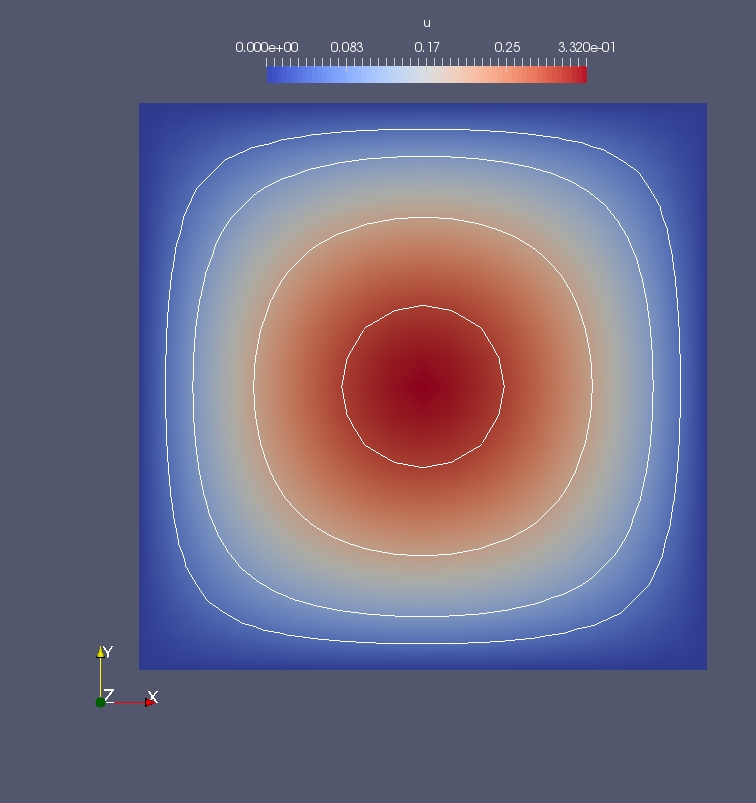
\includegraphics[width=0.7\textwidth]{./cap_mef2d/dados/ex_mef2d_pm/fig_mef2d_pm}
    \caption{Esboço da solução de elementos finitos do problema discutido no Exemplo \ref{ex:mef2d_pm}.}
    \label{fig:mef2d_pm}
  \end{figure}

\ifispython
Com o \fenics, podemos computar a solução deste problema com o seguinte \href{https://github.com/phkonzen/notas/blob/master/src/MetodoElementosFinitos/cap_mef2d/dados/ex_mef2d_pm/ex_mef2d_pm.py}{código}:
\verbatiminput{./cap_mef2d/dados/ex_mef2d_pm/ex_mef2d_pm.py}
\fi
\end{ex}

\subsection*{Exercícios}

\begin{exer}
  Compute uma aproximação de elementos finitos para o seguinte problema
\begin{align}
  -\Delta u &= 10,~x\in (0, 1)\times (0, 1)\\
  u(x,0) &= 0,~0\leq x \leq 1,\\
  u(1,y) &= 0,~0\leq y < 1,\\
  u(x,1) &= 1,~0\leq x \leq 1,\\
  u(0,y) &= 1,~0<x\leq 1.
\end{align}
\end{exer}

\section{Fundamentos da análise de elementos finitos}\label{cap_mef2d_sec_funanlef}

\subsection{Existência e unicidade}

\begin{teo}\normalfont{(Matriz positiva definida)}\label{teo:matriz_definida_positiva}
  A matriz de rigidez é positiva definida.
\end{teo}
\begin{dem}
  A matriz de rigidez $A = [a(\varphi_j,\varphi_i)]_{ij=0}^{n_i-1}$ é obviamente simétrica. Além disso, para todo $\pmb{\xi}\in\mathbb{R}^{n_i}$, $\pmb{\xi}\neq 0$, temos
  \begin{align}
    \pmb{\xi}^TA\pmb{\xi} &= \sum_{i,j=0}^{n_i-1} \xi_ja(\varphi_j,\varphi_i)\xi_i\\
    &= \sum_{i,j=0}^{n_i-1}\xi_j\int_\Omega \nabla \varphi_j\cdot\nabla\varphi_i\,dx\\
    &= \int_\Omega \nabla \left(\sum_{j=0}^{n_i-1}\xi_j\varphi_j\right)\cdot\nabla \left(\sum_{i=0}^{n_i-1}\xi_i\varphi_i\right)\,dx\\
    &= \left\|\nabla \left(\sum_{j=0}^{n_i-1}\xi_j\varphi_j\right) \right\|_{L^2(\Omega)}^2.
  \end{align}
  Portanto, $\pmb{\xi}^TA\pmb{\xi} \leq 0$ e é nulo se, e somente se, $v = \sum_{j=0}^{n_i-1}\xi_j\varphi_j$ for constante. Como $v\in V_{h,0}$, temos que $v$ constante implica $v\equiv 0$, mas então $\pmb{\xi}=0$, o que é uma contradição. Logo, $\pmb{\xi}^TA\pmb{\xi} > 0$ para todo $\pmb{\xi}\in\mathbb{R}^{n_i}$, $\pmb{\xi}\neq 0$.
\end{dem}

\begin{teo}\normalfont{(Existência e unicidade)}
  O problema de elementos finitos \eqref{eq:mef2d_probfem} tem solução única.
\end{teo}
\begin{dem}
  O problema de elementos finitos \eqref{eq:mef2d_probfem} se resume a resolver o sistema linear $A\pmb{\xi} = \pmb{b}$. Do Teorema \ref{teo:matriz_definida_positiva}, temos que $A$ é uma matriz definida positiva e, portanto, invertível. Daí segue, imediatamente, que o problema \eqref{eq:mef2d_probfem} tem solução única.
\end{dem}

\subsection{Estimativa {\it a priori} do erro}

\begin{teo}\normalfont{(Ortogonalidade de Galerkin)}\label{teo:mef2d_orto_Galergin}
  A solução $u_h$ do problema de elementos finitos \eqref{eq:mef2d_probfem} satisfaz
  \begin{equation}
    a(u-u_h,v_h) = L(v_h),~\forall v_h\in V_{h,0},
  \end{equation}
onde $u$ é a solução do problema fraco \eqref{eq:mef2d_probfraco}.
\end{teo}
\begin{dem}
  Segue, imediatamente, do fato de que $V_{h,0}\subset V_0$ e, portanto,
  \begin{equation}
    a(u,v_h) = L(v_h),~\forall v_h\in V_{h,0},
  \end{equation}
bem como
  \begin{equation}
    a(u_h,v_h) = L(v_h),~\forall v_h\in V_{h,0}.
  \end{equation}
\end{dem}

\begin{defn}\normalfont{(Norma da energia.)}
  Definimos a norma da energia por
  \begin{equation}
    \||v|\| := \left(\int_{\Omega} \nabla v\cdot\nabla v\,dx\right)^{1/2} = \|\nabla v\|_{L^2(\Omega)},
  \end{equation}
para todo $v\in V_0$.
\end{defn}

\begin{teo}\normalfont{(Melhor aproximação.)}\label{teo:mef2d_melhor_aprox}
  A solução $u_h$ do problema de elementos finitos satisfaz
  \begin{equation}
    \||u-u_h|\| \leq \||u-v_h|\|,~\forall v_h\in V_{h,0}.
  \end{equation}
\end{teo}
\begin{dem}
  Observando que $u-u_h=u-v_h+v_h-u_h$ e usando a ortogonalidade de Galerkin (Teorema \ref{teo:mef2d_orto_Galergin}), temos:
  \begin{align}
    \||u-u_h|\|^2 &= \int_\Omega \nabla (u-u_h)\cdot\nabla (u-u_h)\,dx\\
    &= \int_{\Omega} \nabla (u-u_h)\cdot\nabla (u-v_h)\,dx + \int_{\Omega} \nabla (u-u_h)\cdot\nabla (v_h-u_h)\,dx\\
    &= \int_{\Omega} \nabla (u-u_h)\cdot\nabla (u-v_h)\,dx\\
    &= \|\nabla (u-u_h)\|_{L^2(\Omega)}^2\|\nabla (u-v_h)\|_{L^2(\Omega)}^2\\
    &= \||u-u_h|\|^2\||u-v_h|\|.
  \end{align}
\end{dem}

\begin{teo}\normalfont{(Estimativa {\it a priori} do erro.)}\label{teo:mef2d_est_apriori_energia}
  A solução $u_h$ do problema de elementos finitos \eqref{eq:mef2d_probfem} satisfaz
  \begin{equation}
    \||u-u_h|\|^2 \leq C\sum_{K\in\mathcal{K}} h_K^2\|D^2u\|_{L^2(K)}^2.
  \end{equation}
\end{teo}
\begin{dem}
  O resultado segue do Teorema da melhor aproximação (Teorema \ref{teo:mef2d_melhor_aprox}) e da estimativa do erro de interpolação (Proposição \ref{prop:interpc}), pois
  \begin{align}
    \||u-u_h|\|^2 \leq \||u-\pi u|\|^2\\
    = \|D(u-\pi u)\|_{L^2(\Omega)}^2\\
    \leq C\sum_{K\in\mathcal{K}} h_K^2\|D^2u\|_{L^2(\Omega)}^2.
  \end{align}
\end{dem}

Para obtermos uma estimativa na norma $L^2(\Omega)$, podemos usar a desigualdade de Poincaré.

\begin{teo}\normalfont{(Desigualdade de Poincaré.)}
  Seja $\Omega\subset \mathbb{R}^2$ um domínio limitado. Então, existe uma constante $C = C(\Omega)$, tal que
  \begin{equation}
    \|v\|_{L^2(\Omega)} \leq C\|\nabla v\|_{L^2(\Omega)},~\forall v\in V_0.
  \end{equation}
\end{teo}
\begin{dem}
  Se $\Omega$ tem contorno suficientemente suave, então existe $\phi$ tal que $-\Delta \phi = 1$ em $\Omega$ com $\sup_{x\in\Omega}|\nabla \phi| < C$. Com isso, temos
  \begin{align}
    \|v\|_{L^2(\Omega)}^2 &= \int_{\Omega} v^2\,dx\\
    &= -\int_{\Omega} v^2\Delta\phi\,dx.
  \end{align}
Agora, usando o Teorema de Green e a desigualdade de Cauchy-Schwarz, obtemos
\begin{align}
  \|v\|_{L^2(\Omega)}^2 &= -\int_{\p\Omega} v^2n\cdot\nabla \phi\,ds + \int_\Omega \nabla v^2\cdot\nabla \phi\,dx\\
  &= \int_\Omega 2v\nabla v\cdot\nabla \phi\,dx\\
  &\leq \sup_{x\in\Omega} |\nabla \phi|\|v\|_{L^2(\Omega)}\|\nabla v\|_{L^2(\Omega)}.
\end{align}
\end{dem}

Com a desigualdade de Poincaré e da estimativa {\it a priori} do erro (Teorema \ref{teo:mef2d_est_apriori_energia}), temos
\begin{equation}\label{eq:mef2d_est_apriori}
  \|u-u_h\|_{L^2(\Omega)} \leq C \||u-u_h|\| \leq Ch\|D^2u\|_{L^2(\Omega)},
\end{equation}
onde $h = \max_{K\in\mathcal{K}} h_K$. Entretanto, esta estimativa pode ser melhorada.

\begin{teo}\normalfont{(Estimativa ótima {\it a priori} do erro.)}
  A solução $u_h$ do problema de elementos finitos \eqref{eq:mef2d_probfem} satisfaz
  \begin{equation}
    \|u-u_h\|_{L^2(\Omega)} \leq Ch^2\|D^2u\|_{L^2(\Omega)}.
  \end{equation}
\end{teo}
\begin{dem}
  Seja $e = u-u_h$ o erro e $\phi$ a solução do problema dual (ou problema adjunto)
  \begin{align}
    -\Delta \phi &= e,~\forall x\in\Omega\\
    \phi &= 0,~\forall x\in\p\Omega.
  \end{align}
Então, usando a fórmula de Green, a ortogonalidade de Galerkin e, então, a desigualdade de Cauchy-Schwarz, temos
\begin{align}
  \|e^2\|_{L^2(\Omega)} &= -\int_\Omega e\Delta\phi\,dx\\
  &=\int_\Omega \nabla e\cdot\nabla\phi\,dx - \int_{\p\Omega} en\cdot\nabla \phi\,ds\\
  &=\int_\Omega \nabla e\cdot\nabla(\phi-\pi\phi)\,dx\\
  \leq\|\nabla e\|_{L^2(\Omega)}\|\nabla(\phi-\pi\phi)\|_{L^2(\Omega)}.
\end{align}
Da estimativa {\it a priori} \eqref{eq:mef2d_est_apriori} (que segue do Teorema \ref{teo:mef2d_est_apriori_energia}) temos
\begin{equation}
  \|\nabla e\|_{L^2(\Omega)} \leq Ch\|D^2u\|_{L^2(\Omega)}.
\end{equation}
Agora, da regularidade elíptica $\|D^2\phi\|_{L^2(\Omega)} \leq C\|\Delta\phi\|_{L^2(\Omega)}$ \cite{Evans1998a} e da estimativa do erro de interpolação (Proposição \ref{prop:interpc}), temos
\begin{equation}
  \|\nabla(\phi-\pi\phi)\|_{L^2(\Omega)} \leq Ch\|D^2\phi\|_{L^2(\Omega)}\leq Ch\|\Delta\phi\|_{L^2(\Omega)} \leq Ch\|e\|_{L^2(\Omega)}.
\end{equation}
Então, temos
\begin{equation}
  \|e\|_{L^2(\Omega)}^2 \leq Ch\|D^2u\|_{L^2(\Omega)}Ch\|e\|_{L^2(\Omega)}.
\end{equation}
\end{dem}

\begin{ex}\label{ex:mef2d_erro}
  Consideremos o seguinte problema de Poisson
  \begin{align}
    -\Delta u &= -2(x_0^2-x_0)-2(x_1^2-x_1),~x\in\Omega:=(0, 1)\times (0, 1),\\
    u &= 0,~x\in\p\Omega.
  \end{align}
  A solução analítica deste problema é $u(x) = (x_0^2-x_0)(x_1^2-x_1)$. Aqui, obtemos aproximações por elementos finitos $u_h$ usando uma malha triangular uniforme $n\times n$ nodos, i.e. $h=1/n$. A Tabela \ref{tab:mef2d_erro} mostra os valores dos erros $\|u-u_h\|_{L^2(\Omega)}$ para diferentes valores de $h$.

  \begin{table}[h!]
    \centering
    \caption{Erros de aproximações por elementos finitos referente ao problema dado no Exemplo \ref{ex:mef2d_erro}.}
    \begin{tabular}{lc|c}
      \#nodos & $h$   & $\|u-u_h\|_{L^2(\Omega)}$ \\\hline
      $10\times 10$   & $1\E-1$  & $9.29\E-4$\\
      $20\times 20$   & $5\E-2$  & $2.34\E-4$\\
      $100\times 100$ & $1\E-3$ & $9.40\E-6$ \\\hline 
    \end{tabular}
    \label{tab:mef2d_erro}
  \end{table}

\ifispython
Com o \fenics, podemos computar a solução deste problema e o erro na norma $L^2$ com o seguinte \href{https://github.com/phkonzen/notas/blob/master/src/MetodoElementosFinitos/cap_mef2d/dados/ex_mef2d_erro/ex_mef2d_erro.py}{código}:
\verbatiminput{./cap_mef2d/dados/ex_mef2d_erro/ex_mef2d_erro.py}
\fi
\end{ex}

\subsection*{Exercícios}

\emconstrucao

%resposta dos exercícios
\ifisbook
%Este trabalho está licenciado sob a Licença Atribuição-CompartilhaIgual 4.0 Internacional Creative Commons. Para visualizar uma cópia desta licença, visite http://creativecommons.org/licenses/by-sa/4.0/ ou mande uma carta para Creative Commons, PO Box 1866, Mountain View, CA 94042, USA.

\chapter*{Resposta dos Exercícios}\label{cap_respostas}
\addcontentsline{toc}{chapter}{Respostas dos Exercícios}

\shipoutAnswer
\fi

%references
\nocite{*}
\bibliographystyle{plain}
\bibliography{main}
\addcontentsline{toc}{chapter}{Referências Bibliográficas}

\ifisbook
\clearpage
\addcontentsline{toc}{chapter}{Índice Remissivo}
\printindex
\fi

\end{document}
